\documentclass[9pt, preprint]{sigplanconf} % <<<

% Keep fontenc and inputenc them in this order.
\usepackage[T1]{fontenc}
\usepackage[latin1]{inputenc}

\usepackage{amsmath}
\usepackage{amssymb}
\usepackage{amsthm}
\usepackage{booktabs}
\usepackage{fancyvrb}
\usepackage{graphics}
\usepackage{microtype}  % do not remove
\usepackage{multirow}
\usepackage{proof}
\usepackage{pygmentize}
\usepackage{rgalg}
\usepackage{tikz}
\usepackage{xcolor}
\usepackage{xspace}

\usepackage{tikz}
\usetikzlibrary{arrows,positioning,fit,backgrounds,shadows,calc}

\usepackage[colorlinks]{hyperref} % keep it last to avoid some warnings

%\g@addto@macro\verbatim{\microtypesetup{activate=false}}

\RecustomVerbatimEnvironment{Verbatim}{BVerbatim}{}
\definecolor{darkred}{rgb}{0.4,0,0}
\definecolor{darkblue}{rgb}{0,0,0.4}
\definecolor{verylightgray}{rgb}{0.9,0.9,0.9}
\definecolor{lightblue}{rgb}{0,0,0.9}
% comment the next line for printing
\hypersetup{colorlinks,linkcolor=darkblue,citecolor=darkblue,urlcolor=darkblue}
\hypersetup{
  pdftitle={Runtime Verification Based on Register Automata},
  pdfauthor={Radu Grigore and Dino Distefano and Rasmus Lechedahl Petersen}}

\title{Runtime Verification Based on Register Automata}
\authorinfo{Radu Grigore \and Dino Distefano}
           {Queen Mary, University of London}
           {\{rgrig,ddino\}@eecs.qmul.ac.uk}
\authorinfo{Rasmus Lerchedahl Petersen}
           {Microsoft Research}
           {a-rapete@microsoft.com}
\authorinfo{Nikos Tzevelekos}
           {Queen Mary, University of London}
           {nikost@eecs.qmul.ac.uk}


\renewcommand{\sectionautorefname}{Section}
\renewcommand{\subsectionautorefname}{\sectionautorefname}

\newcommand{\noterg}[2]{\textcolor{gray}{[\textcolor{red}{#1}: #2]}}
\newcommand{\rg}[1]{\noterg{rg}{#1}}
\newcommand{\rlp}[1]{\noterg{rlp}{#1}}
\newcommand{\dd}[1]{\noterg{dd}{#1}}
\newcommand{\dinocomment}[1]{\dd{#1}}

\newcommand{\B}{\ensuremath{\mathbb{B}}}
\newcommand{\N}{\ensuremath{\mathbb{N}}}
\newcommand{\A}{\ensuremath{\mathcal{A}}}
\newcommand{\delimitVerbatim}{\par\nobreak\medskip\noindent}
\newcommand{\error}{\ensuremath{\textcolor{darkred}{\mathtt{error}}}\xspace}
\newcommand{\eval}[1]{[[#1]]}
\newcommand{\limp}{\Rightarrow}
\newcommand{\pattern}[1]{\ensuremath{\mathtt{\underline{#1}}}}
\newcommand{\pmap}{\rightharpoonup}
\newcommand{\set}[1]{\ensuremath{\mathsf{#1}}}
\newcommand{\start}{\ensuremath{\mathtt{start}}\xspace}
\newcommand{\verbline}[2][]{\[\text{\Verb@#2@}#1\]}

\newcommand{\quoteindent}{1.5\parindent} % could be re-defined before a quote
\newcommand{\eqquote}[2]{{%
  \refstepcounter{equation}\label{#2}%
  \newdimen\qi\qi=\quoteindent
  \setbox0=\vbox{\advance\hsize by-2\qi\noindent\em#1}%
  \newdimen\x\x=\ht0 \advance\x by\dp0%
  \setbox1=\vbox to\x{\vss\hbox{(\arabic{equation})}\vss}%
  \leavevmode\\[1ex]%
  \hbox to\hsize{\hskip\qi\box0\hfil\box1}%
  \\[1ex]}}
\newcommand{\emquote}[1]{{%
  \\[1ex]%
  \newdimen\qi\qi=\quoteindent%
  \hbox to\hsize{\hfil\vbox{\advance\hsize by-2\qi\noindent\em#1}\hfil}%
  \\[1ex]}}

% rg: I tend to give grammars in BFS order
\def\grammar#1{{
  \footnotesize
  \def\b##1{{\rm\Verb@##1@}}\def\*{$^*$}\def\?{$^?$}\def\({$($}\def\){$)$}
  \def\|{$\mid$}\def\+{$^+$}
  \smallskip
  \hbox to\hsize{\hfil\vbox{\halign{\hfil\it##&$\;::=\;$\it##\hfil&\qquad\rm##\hfil\cr#1}}\hfil}
  \smallskip
}}


\newtheorem{lemma}{Lemma}
\providecommand*{\lemmaautorefname}{Lemma}
\newtheorem{proposition}{Proposition}
\newtheorem{theorem}{Theorem}

\theoremstyle{definition}
\newtheorem{definition}{Definition}
\providecommand*{\definitionautorefname}{Definition}
\newtheorem{example}{Example}
\providecommand*{\exampleautorefname}{Example}

\theoremstyle{remark}
\newtheorem{notation}{Notation}
\newtheorem{remark}{Remark}

% For the final version, switch then comment-status of the following lines.
\overfullrule=5pt
%\renewcommand{\noterg}[2]{}

\showboxdepth=10
\showboxbreadth=30
% >>>
\begin{document}
\maketitle
\begin{abstract} % <<<
We introduce a new formal framework aimed at checking temporal safety properties of object-oriented programs.
The underpinning theoretical foundations of our framework is an extended class of {\em register automata}.
As registers' values can be updated, our automata are able to express highly complex properties of systems involving multiple interacting objects.
Specifications are then used to instrument Java bytecode so that their violations can be automatically detected at runtime.
The tradeoff between the coverage and the overhead of the monitoring
system is tunable by means of a number of  parameters.
We have validated our technique by checking several safety properties on large open source projects.

\end{abstract}

% >>>
\section{Introduction} % <<<

Runtime verification is a technique where the behaviour of programs is monitored at runtime to check whether executions
can violate certain safety properties.
Systems for runtime verification stand somehow in between classic verification and testing: they work on the actual system (as testing) but check violations of temporal properties as, for example, it is done in model checking. Compared to traditional formal verification techniques, runtime verification systems check only certain program executions, however, the error reports are accurate and detected violations represent real bugs in the program.

In the context of object-oriented programming  leading runtime verification techniques include JavaMOP~\cite{dblp:journals/sttt/meredithjgcr12}, QVM~\cite{arnold:2008}, Tracematches~\cite{dblp:conf/oopsla/allanachklmsst05}, and techniques based on typestate~\cite{strom1986,dblp:conf/oopsla/bierhoffa07,dblp:conf/oopsla/naeeml08,disney2011,ball2002}. Although powerful,  these methods present some limitations. For example, either   in terms of  language expressivity, or in the ability to express concisely properties of the interaction of several objects 
over time (typestate), or in concisely expressing  properties requiring an unbounded number of different object re-bindings (sometimes called "parameters" in the runtime verification community).

Register Automata~\cite{dblp:conf/focs/kaminskif90} are automata where
a number of registers are used to store and compare data. The values
of registers can be updated over time, and data can be taken from unbounded domains (e.g., the set of object references). Thus register automata provide a powerful device for reasoning about temporal 
relations of a (possibly unbounded) number of objects in a finite manner. They have been studied extensively from the theoretical point of
view and essential results for their analysis have been established (e.g., decidability of emptiness, closure under intersection, and so forth).

Thus, it seems sensible to attempt an approach to runtime verification
taking register automata as the starting point. The aim is to
exploit the flexibility and the power of registers to
address certain properties not easily dealt with in other approaches.
On the formal side, we started from register automata and have extended them driven by typical properties required in real-world object-oriented systems.
The extension has been careful crafted to be able to define the precise mathematical connection with register automata, and yet,
make it easy for programmers to express properties of their code. This process has resulted in the definition of two new classes of 
automata: a high-level and a low-level one. In the high-level automata, temporal properties about programs are naturally expressed. Low-level automata, 
on the other hand, simplify the formal correspondence with  register automata. 
Finally we defined a formal language --- called TOPL (Temporal Object Property Language) --- mapping directly on the 
high-level automata.

We complement the theoretical construction with a practical tool.
We have implemented TOPL  in a runtime parametric verification framework that can be used by Java programmers to express rigorous temporal 
properties about their programs. These properties will then be automatically checked by the system.
The formal correspondence between the properties and register automata
defined in this paper gives a rigorous mathematical foundation to
the approach and allows us to reuse many of the results for register automata on TOPL automata. For example, given a TOPL property, we can decide whether its language is empty.  The formal development is completely hidden from 
the programmer.  
Our system can be tuned  in terms of coverage,  overhead, and trace reporting by means of a number of parameters. 

\paragraph{Contributions.}
In summary, the contributions of this paper are:
\begin{itemize}
\item We define TOPL, a formal specification language tailored to express properties involving object interactions over time in a way that is familiar to object-oriented programmers.
\item We define a precise formal semantics for TOPL, making it suitable for program analysis, both static and dynamic.
\item We define a precise formal correspondence between TOPL automata and register automata. 
In particular we prove that they are equally expressive. As our proof is constructive, this implies that the decidability results for register automata hold also for TOPL automata. Consequently we can decide several features of TOPL specifications (e.g., language emptiness).
\item We have implemented our parametric framework  in a tool that automatically check at runtime violations of TOPL properties in Java programs. A number of parameters are used to tune the precision of the system.

\item We report on experiments of running our tool on large open-source projects. The results are encouraging (e.g., we have found
an interesting and previously unknown  concurrency bug in the DaCapo suite). 
\end{itemize}


The paper is organized as follows.
\autoref{sec:motivating-examples} gives some example properties motivating TOPL.
\autoref{sec:overview} provides background of register automata and defines the basis of our formalism.
\autoref{sec:topl_automata} introduced TOPL automata and proves the equivalence with register automata. 
\autoref{sec:topl} defines the TOPL property language and its semantics.
\autoref{sec:examples} describes several example properties using TOPL.
\autoref{sec:implementation} describes  the implementation of the runtime  verification system.
\autoref{sec:results} discusses the experimental results and \autoref{sec:related}  related work.
Finally, \autoref{sec:conclusions} concludes the paper and describes our plans for future work.

%>>>
\section{Motivating Examples} %<<<
\label{sec:motivating-examples}
Interaction among objects is at the core of the object-oriented paradigm.
Consider for example  Java collections. A typical property one would want to state  is:
\eqquote{If one iterator modifies its collection, then other existing iterators of the same collection become invalid, which means they cannot be used further.}{q:concur-it}
The formalization of the above constraint is non-trivial since it needs to keep track of {\em several objects} (at least two iterators, and one collection) and their {\em interaction over time}.

A slightly more complex scenario is described by classes in Figure~\ref{fig:first.java}.
Class {\tt CharArray} manipulates an array of chars and implements the {\tt Str} interface. 
Class {\tt Concat} is used to concatenate two object of type {\tt Str}. The concatenation implements also the
 {\tt Str} interface. 
Consider the case where {\tt Concat} is used to implement a  {\em rope} data structure.\footnote{ A rope is a binary tree shaped data structure for efficiently storing and manipulating very long strings~\cite{DBLP:journals/spe/BoehmAP95}.} 
Rope's operations like insert, concat, delete may update the shape of the tree and references to its root. 
In this case we may have two (or more) collections {\em sharing} some elements. Consequently iterators operating on these different collections may invalidate each other. We need to modify~\eqref{q:concur-it} increasing its complexity: 
\eqquote{If one iterator modifies its collection, then other existing iterators of collections sharing some elements become invalid, which means they cannot be used further.}{q:concur-it2}

\paragraph{Re-binding of specification variables.}
Now let's consider the case where we want to perform taint checking for input coming from a web form.  What we want to check is the following
property:
\eqquote{Any value introduced by the {\tt input()} method should not
  reach the  {\tt sink()} method without first passing through the {\tt sanitizer()} method.}{q:concur-it3}
This property is at first sight simple. However, it's difficulty can vary depending on the context. Consider in fact the case where
the input is constructed by concatenating strings from the web form, by for example, using ropes implemented with class {\tt Concat}. 
The number of user inputs, and therefore of concatenations, is not known a priori and in general unbounded.
Consequently we will have a possibly unbounded number of tainted objects. 
In a temporal specification we would then need either different logical variables for each different tainted objects or
the ability to {\em re-bind} (or {\em update}) variables in the temporal specification in such a way that at the semantic level we capture all the tainted objects. For an unbounded number of object, re-binding specification variables with
different values during the computation allows the specification to be
kept finite. 

\begin{figure}[t] % first example <<<
%\begin{Verbatim}[commandchars=\\\{\}]
\PY{k+kn}{import} \PY{n+nn}{java.util.*}\PY{o}{;}
\PY{k+kd}{public} \PY{k+kd}{class} \PY{n+nc}{IncorrectIteratorUse} \PY{o}{\PYZob{}}
  \PY{k+kd}{public} \PY{k+kd}{static} \PY{k+kt}{void} \PY{n+nf}{main}\PY{o}{(}\PY{n}{String}\PY{o}{[}\PY{o}{]} \PY{n}{args}\PY{o}{)} \PY{o}{\PYZob{}}
    \PY{n}{List}\PY{o}{<}\PY{n}{Integer}\PY{o}{>} \PY{n}{c} \PY{o}{=} \PY{k}{new} \PY{n}{ArrayList}\PY{o}{<}\PY{n}{Integer}\PY{o}{>}\PY{o}{(}\PY{o}{)}\PY{o}{;}
    \PY{n}{c}\PY{o}{.}\PY{n+na}{add}\PY{o}{(}\PY{l+m+mi}{1}\PY{o}{)}\PY{o}{;} \PY{n}{c}\PY{o}{.}\PY{n+na}{add}\PY{o}{(}\PY{l+m+mi}{2}\PY{o}{)}\PY{o}{;}
    \PY{n}{Iterator}\PY{o}{<}\PY{n}{Integer}\PY{o}{>} \PY{n}{i} \PY{o}{=} \PY{n}{c}\PY{o}{.}\PY{n+na}{iterator}\PY{o}{(}\PY{o}{)}\PY{o}{;}
    \PY{n}{Iterator}\PY{o}{<}\PY{n}{Integer}\PY{o}{>} \PY{n}{j} \PY{o}{=} \PY{n}{c}\PY{o}{.}\PY{n+na}{iterator}\PY{o}{(}\PY{o}{)}\PY{o}{;}
    \PY{n}{i}\PY{o}{.}\PY{n+na}{next}\PY{o}{(}\PY{o}{)}\PY{o}{;} \PY{n}{i}\PY{o}{.}\PY{n+na}{remove}\PY{o}{(}\PY{o}{)}\PY{o}{;} \PY{n}{j}\PY{o}{.}\PY{n+na}{next}\PY{o}{(}\PY{o}{)}\PY{o}{;}
  \PY{o}{\PYZcb{}}
\PY{o}{\PYZcb{}}
\end{Verbatim}

\begin{tiny}
\begin{Verbatim}[commandchars=\\\{\}]
\PY{k+kd}{interface} \PY{n+nc}{Str} \PY{o}{\PYZob{}}
  \PY{k+kt}{void} \PY{n+nf}{set}\PY{o}{(}\PY{k+kt}{int} \PY{n}{i}\PY{o}{,} \PY{k+kt}{char} \PY{n}{c}\PY{o}{)}\PY{o}{;}  \PY{k+kt}{char} \PY{n}{get}\PY{o}{(}\PY{k+kt}{int} \PY{n}{i}\PY{o}{)}\PY{o}{;}
  \PY{k+kt}{int} \PY{n+nf}{len}\PY{o}{(}\PY{o}{)}\PY{o}{;}
  \PY{n}{Itr} \PY{n+nf}{itr}\PY{o}{(}\PY{o}{)}\PY{o}{;}
\PY{o}{\PYZcb{}}
\PY{k+kd}{interface} \PY{n+nc}{Itr} \PY{o}{\PYZob{}}
  \PY{k+kt}{boolean} \PY{n+nf}{hasNext}\PY{o}{(}\PY{o}{)}\PY{o}{;}        \PY{k+kt}{char} \PY{n}{next}\PY{o}{(}\PY{o}{)}\PY{o}{;}
  \PY{k+kt}{void} \PY{n+nf}{set}\PY{o}{(}\PY{k+kt}{char} \PY{n}{c}\PY{o}{)}\PY{o}{;} 
\PY{o}{\PYZcb{}}
\PY{k+kd}{class} \PY{n+nc}{CharArray} \PY{k+kd}{implements} \PY{n}{Str} \PY{o}{\PYZob{}}
  \PY{k+kt}{char} \PY{o}{[}\PY{o}{]} \PY{n}{data}\PY{o}{;}
  \PY{c+c1}{// ...}
\PY{o}{\PYZcb{}}
\PY{k+kd}{class} \PY{n+nc}{Concat} \PY{k+kd}{implements} \PY{n}{Str} \PY{o}{\PYZob{}}
  \PY{n}{Str} \PY{n}{one}\PY{o}{,} \PY{n}{two}\PY{o}{;}
  \PY{k+kd}{public} \PY{k+kd}{static} \PY{n}{Concat} \PY{n+nf}{make}\PY{o}{(}\PY{n}{Str} \PY{n}{one}\PY{o}{,} \PY{n}{Str} \PY{n}{two}\PY{o}{)} \PY{o}{\PYZob{}} \PY{c+cm}{/* ... */} \PY{o}{\PYZcb{}}
  \PY{c+c1}{// ...}
\PY{o}{\PYZcb{}}
\end{Verbatim}

\end{tiny}
\caption{A first example: Java code}
\label{fig:first.java}
\end{figure}
%

The need for rebinding of variables in the specification arises also in other contexts. For example, 
when  reasoning about the evolving shape of dynamically allocated data-structures. 
Consider the following loop using a list:
 \begin{verbatim}
  while (l.next()!=null) {
     // here using the list l in some way...
     ......
  }
\end{verbatim}
If the list {\tt l} is circular or pan-handle shaped, one of the problem could be that the loop will diverge.
Being a violation of a liveness property (termination), divergence cannot be observed at runtime in finite time and therefore it is harder to debug.
If we have obtained the list by calling a third party library, we
would want to check the following property:\footnote{Of course, one
  can write a method (to call before entering the loop) which
  traverses the list and check whether it is circular or
  pan-handle. However, when the scope of the list is not clearly
  defined, these kind of explicit checks become cumbersome and error
  prone.}
\eqquote{The shape of the list should be neither circular nor pan-handle.}{q:concur-it4}
We will see in Section~\ref{sec:examples} that also the encoding of properties of this kind requires the ability to update the 
value of the specification variables.  This is because the way to encode the property is by detecting, when using the list, that we reach some element we have seen before. 

%The following TOPL properties test the shape of a linked list and
%reports an error if it is cyclic or it has the pan-handle shape (i.e.,
%there is a lasso at some point). 
%Directives are omitted.
%%
%\delimitVerbatim
%\begin{Verbatim}[commandchars=\\\{\}]
% property ListNotCyclic
%   start -> start: *
%   start -> a: \pattern{X} := *.getList()
%   a -> a:     \pattern{X} := x.next()
%   a -> b:     \pattern{Y} := x.next()
%   b -> b:     \pattern{Y} := y.next()
%   b -> error: x := y.next()
%   a -> error: x := x.next()
%\end{Verbatim}
%\delimitVerbatim
%The idea is that this property will bind the property variable $x$ with any possible object in the list, and the $y$ with any possible successors (via the next field) of the current binding of $x$.
%Therefore, if there is a lasso, in the list, this will be detected when a new binding of $y$ via a \texttt{b -> b} becomes equal to the binding of $x$.
%The transition \texttt{a ->error} detects the case where there is an object pointing to itself.

%
%The following property detects when a dictionary overwrite one of its bindings.
%\delimitVerbatim
%\begin{Verbatim}[commandchars=\\\{\}]
% property BadDictionary
%   message "dictionary overwrites its bindings"
%   observe <Dictionary.*>
%   prefix <Dictionary>
%   start -> start: *
%   start -> written:   \pattern{D}.put(\pattern{K}, \pattern{V})
%   written -> written: d.put(k, \pattern{V})
%   written -> error:   !v := d.get(k)
%\end{Verbatim}
%\delimitVerbatim
%The overwrite is detected by the guard which checks if the value associated with a key $k$ is the same as the original binding recorded in the property variable $v$.

% >>>
% >>>
\section{Overview and Background}\label{sec:overview} % <<<

\autoref{fig:concepts} shows the main concepts of concern.
Register automata are well-studied devices, introduced decades ago.
The gap between TOPL properties and register automata is filled by two semantic models, namely high-level and low-level TOPL automata.
The high-level model (rollback TOPL automata) is better suited for implementation;
the low-level model (simple TOPL automata) is easier to analyze.

The target of an arrow is at least as expressive as its source.
All three automata models have the same expressivity.
In general, decision problems on automata (such as membership, emptiness, language inclusion), are either decidable for all three models, or undecidable for all three models.
However, decidable problems do not necessarily have the same complexity for the three models.

\begin{figure}[th]\centering
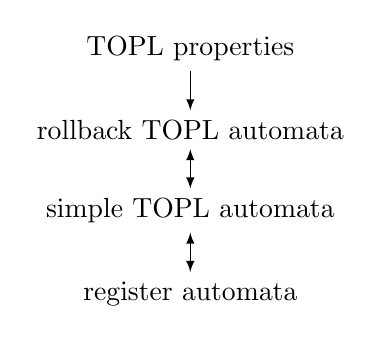
\begin{tikzpicture}[auto,node distance=5mm]
  \node (lang) {TOPL properties};
  \node (rtopl) [below=of lang] {rollback TOPL automata};
  \node (topl) [below=of rtopl] {simple TOPL automata};
  \node (ra) [below=of topl] {register automata};
  \path[draw,->,>=latex]
    (lang) edge (rtopl)
    (rtopl) edge[<->] (topl)
    (topl) edge[<->] (ra);
\end{tikzpicture}
\caption{Main concepts}
\label{fig:concepts}
\end{figure}

We review here register automata and several results about them.
Together with the reductions presented later, these results imply similar results about TOPL automata.

We begin by defining a generic automaton, of which both TOPL and register automata are instances.
A \emph{letter} $\ell$ is an $n$-tuple $(v_1,\ldots,v_n)$ of \emph{values} from a possibly infinite set~$V$;
we denote the \emph{alphabet} by~$\Sigma=V^n$.
A \emph{store} $s$ is an $m$-tuple $(u_1,\ldots,u_m)$ of values;
we denote the set of stores by $S=V^m$.
A \emph{register} $i$ is an integer that identifies a component of the store;
the set of registers is $[m]=\{1,2,\ldots,m\}$.
A \emph{guard} $g$ is a formula in some logic interpreted over pairs of letters and stores;
we write $(s,\ell)\models g$ to denote that store $s\in S$ and the letter $\ell\in\Sigma$ satisfy the guard~$g$, and we denote the set of guards by~$G$.
An \emph{action} $a$ is a small program acting on stores, which has relational semantics;
we denote the set of actions by $A=\Sigma\to(S\times S)$.
Thus, an action applied to a letter $a(\ell)$ is a relation on stores.
We will later specialize to specific and simple logics (for guards) and programming languages (for actions).
A \emph{label} $\lambda$ is a pair $(g,a)$ of a guard~$g$ and an action~$a$;
we denote the set of labels by $\Lambda=G\times A$.

\begin{definition}\label{def:automaton}
An \emph{automaton}~${\cal A}$ with $m$~registers over $n$-tuples of values from the set~$V$ consists of
\begin{itemize}
\item a finite set~$Q$ of states
\item an initial state $q_0\in Q$
\item an initial store $s_0\in S$
\item a set $F\subseteq Q$ of final states
\item a finite transition relation $\delta\subseteq Q\times\Lambda\times Q$
\end{itemize}
\end{definition}

A \emph{configuration}~$x$ is a pair~$(q,s)$ of a state~$q$ and a store~$s$;
we denote the set of configurations by $X=Q\times S$.
The \emph{initial} configuration is $(q_0,s_0)$.
A configuration is \emph{final} when its state is final.
The configuration graph of the automaton is a subset of $X\times\Sigma\times X$.
We write \[x_1\stackrel{\ell}{\to}_{\cal A}x_2\] to mean that $(x_1,\ell,x_2)$ is in the configuration graph of~${\cal A}$.
If the automaton is clear from the context, we omit the subscript.

\begin{definition}\label{def:cgraph}
The \emph{configuration graph} of an automaton consists of exactly those configuration transitions \[ (q_1,s_1) \stackrel{\ell}{\to} (q_2,s_2) \] for which there exists an automaton transition $(q_1,(g,a),q_2)\in\delta$ such that $(s_1,\ell)\models g$ and $(s_1,s_2)\in a(\ell)$.
\end{definition}
An automaton is \emph{nondeterministic} when its configuration graph contains two distinct transitions that have the same source~$x_1$ and are labeled by the same letter~$\ell$:
\[ \text{$x_1\stackrel\ell\to x_2$ and $x_1\stackrel\ell\to x_3$,\quad with $x_2\ne x_3$} \]
Otherwise, the automaton is \emph{deterministic}.

The \emph{language}~${\cal L}({\cal A})$ of an automaton~${\cal A}$ is the set of words that label walks from the initial configuration to some final configuration:
\[ {\cal L}({\cal A}) =
  \{\,\ell_1\ldots\ell_k\mid \text{$x_0$ initial,
  $x_{i-1}\stackrel{\ell_i}\to_{\cal A} x_i$ for $i\in[k]$,
  $x_k$ final}\,\}\]
Being a walk rather than a path, the configurations $x_0$,~$x_1$, \dots,~$x_k$ need not be distinct.

\smallskip

Given a number~$m$ of registers, an arity~$n$ for letters, and a countable set~$V$ of values, the set $A=\Sigma\to(S\times S)$ of actions is uncountable.
Therefore we must focus on a subset of $A$ if we want our automata to be finitely representable.
We will only consider actions that are sequences of assignments.
The assignment $({\sf set}\,i:=j)$ is defined as follows:
\[ \bigl((v_1,\ldots,v_m),(v'_1,\ldots,v'_m)\bigr)\in
  ({\sf set}\,i:=j)\bigl((u_1,\ldots,u_n)\bigr) \]
if and only if $v'_k=v_k$ for all~$k$, except that $v'_i=u_j$.
The sequence operator~$;$ is defined by saying that the relation $(a_1;a_2)(\ell)$ is the composition of the relations $a_1(\ell)$ and $a_2(\ell)$, for all~$\ell$.
The identity action ${\sf nop}$ satisfies ${\sf nop}(\ell)=\{\,(s,s)\mid s\in S\,\}$ for all~$\ell$.

Register automata work with arity $n=1$, that is $\Sigma=V$.
In this case we write $({\sf set}\,i)$ as a shorthand for $({\sf set}\,i:=1)$.
The syntax of guards for register automata is the following:
\begin{align*}
G_{\rm RA} &\;::=\; {\sf fresh} \mid {\sf eq}\,i
\end{align*}
They are interpreted as follows:
\begin{align*}
\bigl((u_1,\ldots,u_m),v\bigr)&\models{\sf fresh}
  &&\text{iff $u_i\ne v$ for all $i$} \\
\bigl((u_1,\ldots,u_m),v\bigr)&\models{\sf eq}\,i
  &&\text{iff $u_i=v$}
\end{align*}

With these notations we can fix a definition for register automata.

\begin{definition}
A \emph{register automaton} with $m$~registers is an automaton over the alphabet $\Sigma=V$ whose labels are given by $\Lambda=\{\,({\sf fresh},{\sf set}\,i)\mid i\in[m]\,\}\cup\{\, ({\sf eq}\,i, {\sf nop})  \mid i\in[m] \,\}$.
\label{def:ra}
\end{definition}

There are several variants of definitions for register automata in the literature.
Our variant corresponds directly to what Neven et al~\cite{dblp:conf/mfcs/nevensv01} call 1N-RA (for `one-way non-deterministic register automata').

\begin{example}\label{ex:ra1}
The language $\{\,abc\mid\text{$a\ne c$ and $b\ne c$}\,\}$ is recognized by the following register automaton with $3$~registers over the alphabet $\Sigma=V\cup\{\bot\}$:
\begin{itemize}
\item $Q=\{1,2,3,4\}$
  and $q_0=1$
  and $s_0=(\bot,\bot,\bot)$
  and $F=\{4\}$
\item the set of transitions is
\begin{align*}\delta =\{ & \bigl(1,({\sf fresh},{\sf set}\,1),2\bigr), \ \bigl(2,({\sf fresh},{\sf set}\,2),3\bigr), \\
& \bigl(2,({\sf eq}\,1,{\sf nop}),3\bigr), \bigl(3,({\sf fresh},{\sf set}\,1),4\bigr) \}.
\end{align*}
\end{itemize}
Observe that:
(1)~The two parallel transitions from 2~to~3 are needed because labels cannot have the shape $({\sf true},{\sf set}\,i)$; in fact, we have not even defined yet the guard {\sf true}.
(2)~Only values from~$s_0$ may appear multiple times in a store; in this case, only~$\bot$.
(3)~Register~3 ensures that $\bot$ will not appear in the third position of words, which is a risk because we extended the alphabet.
(4)~The action of the last transition is superfluous, but required by the definition.
\end{example}

\begin{theorem}\label{th:ra}
The following properties of register automata are known:
\begin{enumerate}
\item The emptiness problem is coNP-complete~\cite{dblp:journals/tcs/sakamotoi00}.
\item The membership problem is NL-complete~\cite{dblp:conf/mfcs/nevensv01} and NP-complete~\cite{dblp:journals/tcs/sakamotoi00}.
\item The inclusion, equivalence, and universality problems are decidable for $2$~registers~\cite{dblp:conf/focs/kaminskif90,dblp:conf/mfcs/nevensv01}.
\item The inclusion, equivalence, and universality problems are undecidable in general~\cite{dblp:conf/mfcs/nevensv01}.
\item Register automata are closed under union, intersection, concatenation, and Kleene star~\cite{dblp:conf/focs/kaminskif90}.
\rlp{Not completely sure if we are talking about the full class.}
\item Register automata are \emph{not} closed under complementation and reversal~\cite{dblp:conf/focs/kaminskif90}.
\rlp{ditto}
\item Nondeterministic register automata are strictly more expressive than deterministic register automata~\cite{dblp:conf/focs/kaminskif90}.
\rlp{ditto\ldots}
\item The language ${\cal L}({\cal A})\cap C^*$ is regular for any register automaton~${\cal A}$ and any finite subset $C\subset V$ of values~\cite{dblp:conf/focs/kaminskif90}.
\end{enumerate}
\end{theorem}

Some of these properties contrast with analogues for finite alphabets, which are better known.
For example with finite alphabets automata are closed under complementation and reversal, and nondeterminism does not increase expressivity.
These results differ for infinite alphabets because registers can be re-bound to different values an unbounded number of times.
On the other hand, once the alphabet is `sliced' to a finite subset, the resulting language is regular in the standard sense.

These results have analogues for TOPL automata.
The details depend on what exactly the arrows from \autoref{fig:concepts} are.
The gist will generally be a transformation of the following kind:
From an automaton~${\cal A}$ in one model, construct an automaton~${\cal A}'$ in another model such that
\[ \ell_1\ldots \ell_k \in {\cal L}({\cal A})
  \iff
f(\ell_1)\ldots f(\ell_k)\in{\cal L}({\cal A}') \]
for some fixed $f$ that is easily computable.
The interesting ideas will be in how ${\cal A}'$~is built;
$f$~handles technicalities.

%>>>
\section{TOPL Automata}\label{sec:topl_automata} % <<<

We now gradually move towards a model that is better suited for runtime verification of Java programs.

\subsection{Simple TOPL Automata} %<<<

TOPL automata work with the alphabet $\Sigma=V^n$ for some~$n\in\N$, unlike register automata, which force $n=1$.
It is then natural to consider different guards and actions, which handle specific components of the letters.
TOPL guards are the following:
\begin{align*}
G_{\rm TOPL} &\;::=\; {\sf eq}\,i=j \\
G_{\rm TOPL} &\;::=\; {\sf neq}\,i\ne j \\
G_{\rm TOPL} &\;::=\; {\sf true} \\
G_{\rm TOPL} &\;::=\; G_{\rm TOPL} \mathrel{\sf and} G_{\rm TOPL}
\end{align*}
If $n=1$, we write $({\sf eq}\,i)$ instead of $({\sf eq}\,i=1)$, and $({\sf neq}\,i)$ instead of $({\sf neq}\,i\ne1)$.
Recall that $({\sf set}\,i)$ abbreviates $({\sf set}\,i:=1)$.
The guards are interpreted as follows:
\begin{align*}
\bigl((u_1,\ldots,u_m),(v_1,\ldots,v_n)\bigr) &\models {\sf eq}\,i=j
  &&\text{iff $u_i=v_j$} \\
\bigl((u_1,\ldots,u_m),(v_1,\ldots,v_n)\bigr) &\models {\sf neq}\,i\ne j
  &&\text{iff $u_i\ne v_j$}
\end{align*}
and
\begin{align*}
(s,\ell) &\models {\sf true}
  &&\text{always} \\
(s,\ell) &\models g_1\mathrel{\sf and} g_2
  &&\text{iff $(s,\ell)\models g_1$ and $(s,\ell)\models g_2$}
\end{align*}

We can now define TOPL automata.

\begin{definition}
A \emph{TOPL automaton} is an automaton whose guards are from the set~$G_{\rm TOPL}$ (defined above) and whose actions are sequences of assignments (defined in \autoref{sec:overview}).
\end{definition}

\begin{example}\label{ex:topl1}
Consider again the language $\{\,abc\mid\text{$a\ne c$ and $b\ne c$}\,\}$.
It is recognized by the following TOPL automaton with $2$~registers over the alphabet $\Sigma=V$:
\begin{itemize}
\item $Q=\{1,2,3,4\}$ and $q_0=1$ and $F=\{4\}$
\item $\delta$ consists of
  $\bigl(1,({\sf true}, {\sf set}\,1),2\bigr)$
  and $\bigl(2,({\sf true}, {\sf set}\,2),3\bigr)$
  and $\bigl(3,({\sf neq}\,1\mathrel{\sf and}{\sf neq}\,2, {\sf nop}),4\bigr)$.
\end{itemize}
Any initial store~$s_0$ works.
\end{example}

It is not difficult to see that TOPL automata are at least as expressive as register automata.

\begin{lemma}[RA to TOPL]\label{lemma:ra-to-topl}
There exists an algorithm that, given a register automaton~${\cal A}$ over the alphabet~$V$, with $m$~registers, $|Q|$~states, and $|\delta|$~transitions, builds a TOPL automaton~${\cal A}'$ over the alphabet $V$, with $m$~registers, $|Q|$~states, and $|\delta|$~transitions such that
\[w\in{\cal L}({\cal A}) \iff w\in{\cal L}({\cal A}') \]
\end{lemma}
\begin{proof}
The guard ${\sf fresh}$ is encoded as the guard ${\sf neq}\,1 \mathrel{\sf and} \ldots \mathrel{\sf and}{\sf neq}\,m$.
All other guards and actions remain unchanged.
\end{proof}

It is relatively harder to establish that TOPL automata are at most as expressive as register automata.

\begin{lemma}[TOPL to RA]\label{lemma:topl-to-ra}
There exists an algorithm that, given a TOPL automaton~${\cal A}$ over the alphabet~$V^n$, with $m$~registers, $|Q|$~states, and $|\delta|$~transitions, builds a register automaton~${\cal A}'$ over the alphabet $V'$, with $m+1$~registers, $O(n\,m^{m+1}|Q|)$~states, and $O(n\,m^{m+2}|\delta|)$~transitions such that
\[\ell_1\ldots \ell_k\in{\cal L}({\cal A}) \iff
  f(\ell_1)\ldots f(\ell_k)\in{\cal L}({\cal A}') \]
where $f\bigl((v_1,\ldots,v_n)\bigr)$ is $v_1\ldots v_n$ repeated $m+1$ times, and $V'$ is~$V$ with up to $m-1$ extra dummy values.
\end{lemma}
\begin{proof}
We describe an encoding chain ${\cal A}_1\to{\cal A}_2\to{\cal A}_3\to{\cal A}_4$ that goes from a TOPL automaton~${\cal A}_1$ to a register automaton~${\cal A}_4$.
The encoding ${\cal A}_2\to{\cal A}_3$ is more difficult than the other two.

\paragraph{Step ${\cal A}_1\to{\cal A}_2$.}
The automaton~${\cal A}_2$ works over the alphabet~$V$, while ${\cal A}_1$ may work on an alphabet~$V^n$ with $n>1$.
The number of registers is preserved.
Each letter $(v_1,\ldots,v_n)$ is transformed into the word $v_1\ldots v_n$ repeated $m+1$ times.
Each transition $\bigl(q_1,(g,a),q_2\bigr)$ is encoded with a path from~$q_1$ to~$q_2$ of length $(m+1)n$.
The first $n$~transitions encode the guard~$g$ -- they are labeled $(g_1,{\sf nop})$, \dots, $(g_n,{\sf nop})$.
The guard~$g_j$ contains the conjunct ${\sf eq}\,i$ if and only if $g$~contains the conjunct ${\sf eq}\,i=j$; similarly for ${\sf neq}$.
The following $mn$~transitions encode the action~$a$ -- they are labeled $({\sf true}, a_1)$, \dots, $({\sf true}, a_{mn})$.
If the last assignment of~$a$ to register~$i$ is ${\sf set}\,i:=j$, then $a_{(i-1)m+j}$ is ${\sf set}\,i$.
Otherwise, if $a$ does not assign at all to register~$i$, then $a_{(i-1)m+1}$ is ${\sf nop}$.

The labels of~${\cal A}_2$ have one of the following shapes:
\begin{itemize}
\item $({\sf eq}\,i_1\mathrel{\sf and}{\sf eq}\,i_2\ldots
  \mathrel{\sf and}{\sf neq}\,i'_1\mathrel{\sf and}{\sf neq}\,i'_2\ldots,\;
  {\sf nop})$
\item $({\sf true},\;{\sf set}\,i)$
\item $({\sf true},\;{\sf nop})$
\end{itemize}
If automaton~${\cal A}_1$ has $|Q|$~states and $|\delta|$~transitions, then ${\cal A}_2$ has $O(mn|Q|)$~states and $O(mn|\delta|)$~transitions.

\paragraph{Step ${\cal A}_2\to{\cal A}_3$.}
Again, the number of registers is preserved. For this step, the
transformation of letters is the identity.
The automaton~${\cal A}_3$ uses guards from~$G_{\rm RA}$, while ${\cal A}_2$ uses guards from~$G_{\rm TOPL}$.
Observe that a register automaton never stores a value twice, because assignments are guarded by ${\sf fresh}$.
This is the main obstacle.
The key idea of the encoding ${\cal A}_2\to{\cal A}_3$ is the following:
\emquote{Encode a function $r\in[m]\to[m]$ in the state itself such that $r(i)$ is the register of~${\cal A}_3$ that currently simulates the register~$i$ of~${\cal A}_2$.
If two registers $i\ne j$ of~${\cal A}_2$ hold the same value, they are simulated by the same register $r(i)=r(j)$ of~${\cal A}_3$.}
Let us develop the idea in some detail.
Let $m$~and~$Q$ denote the count of registers and, respectively, the set of states of~${\cal A}_2$.
The set of states of~${\cal A}_3$ is~$Q\times([m]\to[m])$.
Each state~$q$ of~${\cal A}_2$ is encoded with $m^m$ states $(q,r)$ of~${\cal A}_3$.
The configuration $\bigl((q,r),(u_1,\ldots,u_m)\bigr)$ of~${\cal A}_3$ simulates the configuration $\bigl(q,(v_1,\ldots,v_m)\bigr)$ of~${\cal A}_2$ with $v_i=u_{r(i)}$.
Moreover, we ensure that no two registers of~${\cal A}_3$ hold the same value;
that is, the stores of~${\cal A}_3$ are injective, $u_i\ne u_j$ if $i\ne j$.
To ensure that the initial store of~${\cal A}_3$ is injective we may need to use up to $m-1$ dummy values.

Each transition $\bigl(q_1,(g,a),q_2\bigr)$ of~${\cal A}_2$ is encoded into several transitions $\bigl((q_1,r),(g',a'),(q_2,r')\bigr)$ of~${\cal A}_3$.
Here $r$ takes all $m^m$ possible values, and $g'$,~$a'$, and~$r'$ are chosen depending on $g$,~$a$, and~$r$, as described below.

\smallskip
Consider a transition $\bigl(q_1,({\sf eq}\,i_1\mathrel{\sf and}{\sf eq}\,i_2\mathrel{\sf and}\ldots\mathrel{\sf and}{\sf neq}\,i'_1\mathrel{\sf and}{\sf neq}\,i'_2\mathrel{\sf and}\ldots,{\sf nop}),q_2\bigr)$.
Let $I=\{\,i_1,i_2,\ldots\,\}$ and $I'=\{\,i'_1,i'_2,\ldots\,\}$.
Note that transitions labeled by $({\sf true},{\sf nop})$ are a special case.
We analyze separately the cases $I=\emptyset$ and $I\ne\emptyset$.

\emph{Case $I=\emptyset$}.\quad
The guard requires the current letter~$\ell$ to be different from the values in the set~$I'$ of registers of~${\cal A}_2$.
So, $\ell$~must be different from the values held in the set~$r(I')$ of registers of~${\cal A}_3$.
Because the stores of~${\cal A}_3$ have no repeated value, $\ell$ may be either fresh, or equal to a register outside of the set~$r(I')$.
Thus, the encoding consists of several parallel transitions from~$(q_1,r)$ to~$(q_2,r)$.
One is labeled $({\sf fresh},{\sf nop})$, and several are labeled $({\sf eq}\,j,{\sf nop})$ for each $j\in[m]-r(I')$.

\emph{Case $I\ne\emptyset$.}\quad
The guard also requires that the current letter equals the value in the set~$I$ of registers of~${\cal A}_2$.
This cannot be true if $|r(I)|>1$ or $r(I)\cap r(I')\ne\emptyset$: The encoding in this case is no transition.
Otherwise, $r(I)=\{i\}$ for some~$i$, and the encoding is a transition from~$(q_1,r)$ to~$(q_2,r)$ labeled by $({\sf eq}\,i,{\sf nop})$.

\smallskip
Consider a transition $\bigl(q_1,({\sf true},{\sf set}\,i),q_2\bigr)$.
Either the current letter is in some register or it is in none.
To account for the first case, the encoding contains parallel transitions from~$(q_1,r)$ to $(q_2,r'_j)$ labeled by $({\sf eq}\,j,{\sf nop})$, for all $j\in[m]$.
Here $r'_j$~is the same as~$r$ except that $r'_j(i)=j$.
To account for the second case, the encoding contains a transition from~$(q_1,r)$ to~$(q_2,r'_j)$ labeled by $({\sf fresh},{\sf set}\,j)$, for one~$j$ chosen as follows.
If $r$ is a permutation then $j=r(i)$; otherwise $j$ is any element of $[m]-r([m])$.

\smallskip
If automaton~${\cal A}_2$ has $|Q|$~states and $|\delta|$~transitions, then ${\cal A}_3$ has $O(m^m|Q|)$~states and $O(m^{m+1}|\delta|)$~transitions.

\paragraph{Step ${\cal A}_3\to{\cal A}_4$.}
Transitions labeled by $({\sf fresh},{\sf nop})$, which are produced by the encoding described so far, are not allowed in register automata.
They can be handled by adding one register, without significantly increasing the number of transitions.
First, each label $({\sf fresh},{\sf nop})$ is transformed into $({\sf fresh},{\sf set}\,m+1)$.
Second, for each transition labeled $({\sf fresh},a)$, we add a parallel transition labeled $({\sf eq}\,m+1,a)$.
Again, the transformation of letters is the identity.

If the automaton~${\cal A}_3$ has $m$~registers and $|\delta|$~transitions, then ${\cal A}_4$~has $m+1$~registers and $O(|\delta|)$ transitions.

\smallskip
This completes the proof.
\end{proof}

\begin{remark}
It follows from \autoref{lemma:ra-to-topl} and \autoref{lemma:topl-to-ra} that simple TOPL automata and register automata are equally expressive.
\end{remark}

%>>>
\subsection{Automata with Rollback and Skip} %<<<

TOPL automata are almost convenient for runtime verification of Java.
The letters will be events like method calls and returns.
Calls and returns happen, strictly speaking, at different moments.
Moreover, some properties might explicitly mention other events that must happen between a call and its corresponding return.
But, consider the constraint that iterators should advance only if {\tt hasNext} returned {\tt true}.
The event `{\tt hasNext} was called on the iterator that is being tracked' and the event `{\tt hasNext} returned {\tt true}' are distinct.
Yet, it is convenient to pretend that two such consecutive events make one composed event.
This motivates rollback, a mechanism by which transitions consume multiple consecutive letters.

\begin{definition}\label{def:rollback}
A \emph{rollback automaton}~${\cal A}$ consists of:
\begin{itemize}
\item a finite set~$Q$ of states; an initial state $q_0\in Q$; an initial store $s_0\in S$; a set $F\subseteq Q$ of final states
\item a finite transition relation $\delta\subseteq Q\times\Lambda^*\times Q$
\end{itemize}
where $\Lambda$ is a set of labels as defined in \autoref{sec:overview}.
\end{definition}

The difference between rollback automata and (simple) automata, according to definitions \ref{def:automaton}~and~\ref{def:rollback}, is that rollback transitions have a list of labels $\bar\lambda=\lambda_1\ldots\lambda_d$, while simple transitions have exactly one label~$\lambda$.
A transition with exactly one label is said to be a \emph{unit transition}.
If a rollback automaton has only unit transitions, then it is also a (simple) automaton.

The semantics of a rollback automaton cannot be described by the configuration graph from \autoref{def:cgraph}, because that definition does not handle non-unit transitions.
Instead, we define a rollback configuration graph.
Perhaps surprisingly, in the case of simple automata, the rollback configuration graph does not coincide with the configuration graph.
This discrepancy is explained by the different goals of the two models: automata without rollback are meant to be easy to analyze, while rollback automata are meant to be convenient for specifying properties of object-oriented programs.
Often the desired behavior for a letter is to remain in the same configuration.
Without rollback, this behavior is achieved by explicit loops in the automaton.
The definition of the rollback configuration graph reduces the need to explicitly list such skip loops.

A \emph{rollback configuration} is a pair~$(x,w)$ of a configuration~$x$ and a word~$w$;
we denote the set of rollback configurations by $Y=X\times\Sigma^*$.
We think of $w$ as ``yet to be processed''.
A rollback configuration is \emph{initial} when its configuration is the initial configuration; that is, it has the shape $\bigl((q_0,s_0),w\bigr)$, where $q_0$~is the initial state of the automaton, and $s_0$~is the initial store of the automaton.
A rollback configuration is \emph{final} when its state is final and its word is the empty word; that is, it has the shape $\bigl((q,s),\epsilon\bigr)$, where $q$~is one of the final states~$F$ of the automaton, and $\epsilon$~is the empty word.
The rollback configuration graph is a subset of $Y\times\Sigma^*\times Y$.
We write \[ y_1 \stackrel w\hookrightarrow_{\cal A} y_2\] to mean that $(y_1,w,y_2)$ is in the rollback configuration graph of~${\cal A}$.
If the automaton is clear from the context, we omit the subscript.

The following concepts simplify the definition of the rollback configuration graph.
The (simple) automaton \[{\cal T}\bigl(s_0;(g_1,a_1),\ldots,(g_d,a_d)\bigr)\] is defined to have states $0$,~$1$, \dots,~$d$, out of which $0$~is initial and $d$~is final, transitions $\bigl(i-1,(g_i,a_i),i\bigr)$ for all $i\in[d]$, and initial store~$s_0$.
Recall that $\ell_1\ldots\ell_k\in{\cal L}({\cal A})$ when there exist (not necessarily distinct) configurations $x_0$,~$x_1$, \dots,~$x_k$ such that $x_0$~is the initial configuration, $x_k$~is a final configuration, and \[x_{i-1}\stackrel{\ell_i}\to_{\cal A}x_i\qquad\text{for $i\in[k]$}\]
When the store of~$x_k$ is~$s_k$ we say that \emph{${\cal A}$ can accept $\ell_1\ldots\ell_k$ with store~$s_k$}.
A word may be accepted with multiple stores.

\begin{definition}\label{def:rcg}
The \emph{rollback configuration graph} of an automaton consists of two types of transitions:
\begin{enumerate}
\item \emph{rollback transitions}
  \[\bigl((q_1,s_1),ww'\bigr)\stackrel w\hookrightarrow\bigl((q_2,s_2),w'\bigr)\]
when there exists a transition $(q_1,\bar\lambda,q_2)\in\delta$ such that ${\cal T}(s_1;\bar\lambda)$ can accept $w$ with store~$s_2$
\item \emph{skip transitions}
  \[(x,\ell w)\stackrel\ell\hookrightarrow(x,w)\]
when no rollback transition starts from $(x,\ell w)$
\end{enumerate}
\end{definition}

The \emph{rollback language}~${\cal L}_\rho({\cal A})$ of an automaton~${\cal A}$ is the set of words that label walks from some initial rollback configuration to some final rollback configuration:
\begin{multline*}
{\cal L}_\rho({\cal A})=\\ 
  \{\,w_1\ldots w_k\mid
    \text{$y_0$~initial,
    $y_{i-1}\stackrel{w_i}\hookrightarrow y_i$ for $i\in[k]$,
    $y_k$~final}\,\}
\end{multline*}
Since a simple automaton~${\cal A}$ is also a rollback automaton, is has both a simple language~${\cal L}({\cal A})$ and a rollback language~${\cal L}_\rho({\cal A})$.
The treatment of skip transitions implies the aforementioned
discrepancy, that the languages ${\cal L}({\cal A})$ and ${\cal L}_\rho({\cal A})$ are usually distinct.

\begin{example}
Consider the automaton consisting of one transition labeled with the guard ${\sf eq}\,1$, from the initial state to the final state.
The alphabet is $\Sigma=V$ and the initial store has one register containing value~$v$.
The simple language of this automaton consists of one word made of one letter, namely~$v$.
The rollback language, on the other hand, consists of all words that contain the letter~$v$.
\end{example}

It is possible, however, to transform TOPL automata such that their rollback languages coincide with their simple languages.

\begin{lemma}[TOPL to rTOPL]\label{lemma:topl-to-rtopl}
There exists an algorithm that, given a TOPL automaton~${\cal A}$ with $|Q|$~states, at most $d$~transitions outgoing of each state, and guards with at most $k$~conjuncts, builds a TOPL automaton~${\cal A}'$ with $|Q|+1$ states and at most $(d+k^d)|Q|$ transitions such that
\[ w\in{\cal L}({\cal A}) \iff w\in{\cal L}_\rho({\cal A}')\]
\end{lemma}
\begin{proof}
For the simple automaton~${\cal A}$ compare the simple configuration graph with the rollback configuration graph.
Each simple transition $x_1\to^\ell x_2$ corresponds to several rollback transitions $ (x_1,\ell w)\hookrightarrow^\ell (x_2,w)$, for all $w$.
The rollback graph, however, also has skip transitions $(x,\ell w)\hookrightarrow^\ell (x,w)$ for configurations~$x$ that have no outgoing rollback transitions.
Thus, the simple language and the rollback language would agree if all simple configurations would have at least one outgoing simple transition.

We obtain ${\cal A}'$ from~${\cal A}$ by adding unit transitions that do not change the simple language, but ensure that all simple configurations have an outgoing transition.
First we add a special stuck state~$q_{\rm stuck}$.
Then, for each original state~$q$, we list the guards $g_1$,~$g_2$, \dots,~$g_d$ of the outgoing transitions.
The configuration $(q,s)$ has no outgoing transition for some~$\ell$ when $(s,\ell)\not\models g_i$ for $i\in[k]$.
So, we synthesize a guard~$g$ that holds exactly in this situation.
Informally, we want to add a transition from~$q$ to~$q_{\rm stuck}$ with the guard $g=\lnot g_1\land\ldots\land\lnot g_d$ and the action ${\sf nop}$.
There is one small complication: $G_{\rm TOPL}$ does not have a negation operator.
However, we can negate the simple guards ${\sf eq}$ and ${\sf neq}$, we can use distributivity to put $g$ in disjunctive normal form, and we can simulate disjunction by parallel transitions.
Thus, if each $g_i$ contains up to $k$ simple conjuncts, we add at most $k^d$ transitions from state~$q$.
\end{proof}

The converse transformation is more difficult.
There are many obvious ways to simulate a rollback TOPL automaton with a simple TOPL automaton, and many of them are wrong.
Note, for example, that when the set~$V$ of values is countable, the simple configurations are countable, but the rollback configurations are uncountable.
Rollback, which ensures that several letters occur atomically, and skip, which filters irrelevant letters, usually lead to intuitive behaviors, but not always, as the following example illustrates.

\begin{example}
Consider the following rollback TOPL automaton with $2$~registers over the alphabet $\Sigma=V=\{A,B\}$:
\begin{itemize}
\item $Q=\{1,2,3\}$ and $q_0=1$ and $s_0=(A,B)$ and $F=\{3\}$
\item $\delta$ consists of $\bigl(1,\bigl[({\sf eq}\,2,{\sf nop}),({\sf eq}\,1,{\sf nop}),({\sf eq}\,2,{\sf nop})\bigr],2\bigr)$ and $\bigl(1,\bigl[({\sf eq}\,1, {\sf nop})\bigr],3\bigr)$
\end{itemize}
The rollback language of this is automaton consists of those words in which the first $A$ is not surrounded by two $B$s.
For example it contains $A$, $BA$, $BAA$, and $BAAB$, but not $BAB$ or~$BBAB$.
\end{example}

The key idea for encoding rollback TOPL automata into simple TOPL automata is the following:
\emquote{It is sufficient to simulate rollback configurations with words shorter than the length~$d$ of the longest transition, because both rollback and skip transitions depend on $\le d$~letters.}
If $|w|<d$, it should be possible to encode a rollback configuration $((q,s),w)$ using the finite memory of a simple TOPL automaton.
To decide which transitions to take we have $|w|+1$ letters, the ones stored in the current configuration plus the current letter, and $m$~registers to consider.
If $|w|+1<d$, then the current letter~$\ell$ is simply stored in the current configuration, and we move to (the encoding of) $((q,s),w\ell)$.
Eventually, $d$~letters are available and all transitions outgoing from~$q$ can be evaluated.
The original guards involve comparing letter components with register values.
Now some of the letter components are themselves in registers, and TOPL automata do not have guards that compare registers.
But, we can ensure that the stores are injective (as in the translation from TOPL automata to register automata) and then the information about which registers equal which registers is statically available.
Actions simply translate to substitutions into latter guards on the same transition.

\begin{lemma}[rTOPL to TOPL]\label{lemma:rtopl-to-topl}
There exists an algorithm that, given a rollback TOPL automaton~${\cal A}_\rho$ over the alphabet~$V_\rho^n$ with $m_\rho$~registers, $|Q_\rho|$~states, and $|\delta_\rho|$~transitions of length~$\le d$, builds a simple TOPL automaton~${\cal A}$ with $m=m_\rho+dn$ registers, $O(d(d+1) (m+1)^m|Q_\rho|)$ states, and $O(d(d+1) (m+1)^{(m+n)}|\delta_\rho|)$ transitions such that
\[ w\in{\cal L}_\rho({\cal A}_\rho) \iff w\underbrace{\ell_\bot\ldots\ell_\bot}_{\text{$d+1$~times}}\in{\cal L}({\cal A})\]
where $\ell_\bot$ is an extra dummy letter.
\end{lemma}
\begin{proof}
The set of states of~${\cal A}$ is \[Q=Q_\rho\times\{0,\ldots,d\}\times\{0,\ldots,d-1\}\times\bigl([m]\pmap[m]\bigr)\]
When the rollback configuration
\[ \bigl(q_\rho,(v_1,\ldots,v_{m_\rho})\bigr),\ell_0\ldots\ell_{h-1}\]
of~${\cal A}_\rho$ is reached, one of the simple configurations
\[ (q_\rho,h,k,r),\;(u_1,\ldots,u_m) \]
of~${\cal A}$ is reached.
Here $h$~is the length of the remembered history, while $k$,~$r$, $u_1$, \dots,~$u_m$ vary subject to the following constraining invariants:
\begin{itemize}
\item the stores of~${\cal A}$ are injective: $u_i \ne u_j$ if $i\ne j$
\item for $i\in[m_\rho]$, the value of register~$i$ of~${\cal A}_\rho$ is stored in register $r(i)$ of~${\cal A}$; that is, $ u_{r(i)} = v_i $
\item for $0\le k'<h$ and $\ell_{k'}=(v'_1,\ldots,v'_n)$ and $1\le i'\le n$, the $i'$th component~$v'_{i'}$ of letter~$\ell_{k'}$ is stored in register $r(\iota(k+k',i'))$ of~${\cal A}$, where $\iota(k'',i')=m_\rho+(k''\bmod d)n+i'$; that is,
  \[u_{r(\iota(k+k',i'))}=v'_{i'}\]
\item $r$ is undefined for register slots that are reserved for storing letters but are currently unused; namely, $r(\iota(k+k',i'))$ is undefined for all $i'$~and~$k'$ such that $1\le i'\le n$ and $h\le k'<d$
\end{itemize}

\smallskip
We consider in turn each state $q=(q_\rho,h,k,r)$.
Its outgoing transitions are determined by the outgoing transitions of~$q_\rho$.

{\it Case $h<d$}.
In this case all outgoing transitions of~$q$ simply record the current letter $\ell=(v_1,\ldots,v_n)$.
To maintain the injectivity of stores, only those components of~$\ell$ that are not already in some register must be stored.
We consider $(m+1)^n$ distinct situations: each of the $n$~components may be in one the $m$~registers, or it may be fresh.
Such a situation is described by a function $p\in[n]\pmap[m]$.
We add to~${\cal A}$ a transition
\[ (q_\rho,h,k,r),\;(g_p,a_p),\;(q_\rho,h+1,k,r_p)\]
The guard~$g_p$ is constructed such that it ensures we are indeed in a situation described by~$p$; the action~$a_p$ stores the fresh values of~$\ell$ somewhere outside of $r([m])$; the function~$r_p$ records where the fresh values were stored and where the existing values already were.

The guard $g_p$ is constructed as follows.
If $p(j)$ is undefined, which means that $v_j$ should be fresh, then $g_p$ contains conjuncts $({\sf neq}\,i\ne j)$ for $i\in[m]$.
If $p(j)$ is defined, which means that $u_{p(j)}=v_j$, then $g_p$ contains the conjunct $({\sf eq}\,p(j)=j)$.
These are all the conjuncts of~$g_p$.

We now fix some injection $\sigma$ from the set $\{v_j\mid\text{$p(j)$ undefined}\}$ of fresh values to the set $[m]-r([m])$ of unused registers.
The action $a_p$ contains an assignment $({\sf set}\,\sigma(v_j):=j)$ for each $j$ where $p(j)$~is undefined.
Also
\[ r_p(\iota(k',i')) = \begin{cases}
  p(i')  & \text{if $k'=k+h$ and $p(i')$ defined} \\
  \sigma(v_{i'}) & \text{if $k'=k+h$ and $p(i')$ undefined} \\
  r(\iota(k',i')) &\text{otherwise}
\end{cases}\]


{\it Case $h=d$}.
At this point the values in the $m$~registers of~${\cal A}$ are enough to decide whether to simulate a rollback or a skip transition of~${\cal A}_\rho$.
(Note that we could use the current letter and decide one step earlier, when $h=d-1$, which transitions to take.
But, that alternative is slightly more complex.)
First we encode the transitions outgoing from~$q_\rho$,
\[ (q_\rho, [(g_0,a_0),\ldots,(g_{d'-1},a_{d'-1})], q'_\rho)
  \qquad\text{with $d'<d$} \]
and later we will encode the skip configuration transition.

Consider an assignment $({\sf set}\,i:=j)$ that appears in~$a_{k'}$.
Suppose that the distribution of values just before this assignment is given by~$r'$.
This means that the register~$i$ of~${\cal A}_\rho$ is simulated by $r'(i)$, and that the $j$th component of letter~$\ell_{k'}$ is simulated by $r'(\iota(k+k',j))$.
After the assignment is executed, the distribution of values is given by
\[r''(i') = \begin{cases}
  r'(\iota(k+k',j)) & \text{if $i'=i$} \\
  r'(i') & \text{otherwise}
\end{cases}\]
Thus, it is possible to find the register distribution function after each of the $d'$~steps.
Let us write $r_{k'}$ for the distribution function just before step~$k'$; in particular, $r_0=r$, where $r$~is given by the state~$q$ of~${\cal A}$.
Suppose now that $g_{k'}$ contains the conjunct $({\sf eq}\,i=j)$.
We can evaluate this conjunct statically by checking whether $r_{k'}(i)=r_{k'}(\iota(k+k',j))$.
Similarly, we can evaluate all guards $g_0$,~$g_1$, \dots,~$g_{d'-1}$.
If some guard does not hold, then the encoding is nothing.
If all guards hold, then we add outgoing transitions.
These transitions must also save the current letter, so the whole process from {\it Case $h<d$} is repeated.
However, that process is applied as if the starting state has the value distribution function $r_{d'}$, rather than~$r$; as if the history is $h-d'$, rather than~$h$; and as if the reference point is $(k+d')\bmod d$, rather than~$k$.

If the state $q=(q_\rho,d,k,r)$ still has no outgoing transitions at this point, it is because none of the outgoing transitions of~$q_\rho$ have guards that all hold.
In this case, we must simulate a skip transition.
This is done as in {\it Case $h<d$}, except we first simulate removing the letter to which $k$ points.
We do so by incrementing~$k$ and decrementing~$h$ and
 replacing the distribution function~$r$ by one that is undefined at $\iota(k,i')$ for $i'\in[n]$.

\smallskip
Finally, we add one final state, and transitions to it from the states with $h=d$.
These transitions have a guard that requires all $d$ saved letters to be~$\ell_\bot$.
\end{proof}

\begin{remark}
It follows from \autoref{lemma:topl-to-rtopl} and \autoref{lemma:rtopl-to-topl} that rollback TOPL automata and simple TOPL automata are equally expressive.
\end{remark}

%>>>
\subsection{Properties} %<<<

The following are consequences of \autoref{th:ra} and Lemmas \ref{lemma:ra-to-topl},~\ref{lemma:topl-to-ra}, \ref{lemma:topl-to-rtopl}, and~\ref{lemma:rtopl-to-topl}.

\begin{theorem}\label{th:main}
Register automata, simple TOPL automata, and rollback TOPL automata share the following properties:
\begin{enumerate}
\item The emptiness and the membership problems are decidable.
\item The language inclusion, the language equivalence, and the universality problems are decidable for $1$~register.
\item The language inclusion, the language equivalence, and the universality problems are undecidable in general.
\item The languages of these automata are closed under union, intersection, concatenation, and Kleene star.
\item The languages of these automata are not closed under complementation.
\end{enumerate}
\end{theorem}

% >>>
% >>>
\section{TOPL Properties}\label{sec:topl} % <<<

In this section, we describe the user level language of TOPL
properties, as well as the translation from TOPL properties to
rollback TOPL automata in \autoref{fig:concepts}.
%
This language provides a user-friendly way to write down certain
rollback TOPL automata.
As such, TOPL properties form a subset of rollback TOPL
automata, and the translation in \autoref{fig:concepts} is morally an
injection. There is, however, in the interest of user-friendliness,
some encoding happening.

Syntactically, a TOPL property has a set of transitions.\footnote{For
  the complete BNF grammar for TOPL we refer to~\cite{our-fool2011}.}
Each transition is a labelled arc (directed edge) with a source and a
target vertex identified by their name.
There must be a vertex named \start and one named \error.
Labels look like method calls.

In the following, we will describe TOPL labels and how they translate to guards
and actions. But first we will describe the events that a TOPL
property considers and hence the alphabet that the corresponding
rollback TOPL automaton works over.

\subsection{The Alphabet}

We model the semantics of programs and properties as sets of event
traces. We say that a program \emph{violates} a property when their sets of traces intersect.
In other words, properties encode bad executions, rather than good executions.

The traces of events that a property $P$ deems lead to a bad execution is thus the language
of the corresponding automaton $\A_P$. Observable events for TOPL properties are method calls
with parameter values and a time-tag. The method name is taken to be a
string literal and an arity (for simplicity we do not distinguish
overloaded methods with the same arity). The time-tag is either $call$ or $ret$,
corresponding to observing the method being called or returned
from. If the time-tag is $ret$, the event carries the return value
rather than any parameter values.

Thus, for $\A_P$, the values of interest come from two
sources; event ids and parameter values: The set $E$ of event ids is given by
the grammar
\[
call\ m^k \mid return\ m^k
\]
where $m^k$ is one of the method names mentioned in $P$ (with arity~$k$).

The set $V_L$ of possible parameter values is the set of values from
the programming language (e.g., Java)
plus a dummy value $\bot$.

The values are then $V = E + V_L$, and the alphabet is $V^{n+2}$,
where $n$ is the maximal arity of a method mentioned in $P$.
(We need one extra register for the return value and one for the event
id.)

We are only concerned with the subset $E \times V_L^{n+1}$, ie the
tuples where exactly the first component is an event
id. If $P$ has a maximal arity of 5, the event $call\ m^3(a, b, c)$
would be understood as $(call\ m^3, \bot,  a, b, c, \bot, \bot)$ by
$\A_P$. Here the first component is the event id, the second is a
filler for the return value, the next three are the parameter values and the rest are
fillers which allows all tuples to have the same lenght. The event $ret\ r = m^3$
would be understood as $(ret\ m^3, r, \bot, \bot, \bot, \bot, \bot)$ by
$\A_P$.

We can now describe the labels of $P$ and explain how they are transformed into guards and
actions of $\A_P$.

\subsection{Guards and Actions from Labels}

Labels refer to the registers via \emph{patterns}. To retain the
flavour of a programming language, we call the registers of $P$
\emph{property variables}.
%
For each property variable \Verb@v@ there are three associated patterns.
The uppercase pattern \Verb@V@ matches any value and writes it in the property variable \Verb@v@.
The lowercase pattern \Verb@v@ reads the value of the property variable \Verb@v@ and only matches that value.
The negated lowercase pattern \Verb@!v@ reads the value of the
property variable \Verb@v@ and only matches different values.

Further, every element of $V$ acts as a pattern that matches only the value it denotes,
and a wildcard~* pattern matches any value.

\smallskip
A TOPL property is \emph{well-formed} when it satisfies the following two conditions:
{\em (i)} labels must contain uppercase value patterns at most once; {\em (ii)}
any use of a lowercase patterns must be preceded by a use of the corresponding uppercase pattern on all paths from \start  (i.e., property variables must be written before being read).
From now on we assume TOPL properties to be well-formed.

A label is of one of three forms:
\[
  l ::=
  call\;m^k(x_1, \ldots, x_k) \mid
  ret\;x := m^k \mid
  x := m^k(x_1, \ldots, x_k)
\]
where $x$ and $x_1, \ldots, x_k$ are all patterns.
The first two forms describe observable events and will be translated
into unit transitions. We describe that translation first and treat
the last form at the end.

In order to match elements from $V$, there is an extra register in
$\A_P$ for each unique element mentioned by $P$ (note that this
includes all the method names). This register contains
that value in the initial state of $\A_P$ and is never overwritten.

For each pattern $x$ which is not *, we define three functions:
$reg(x) : \N$ gives the associated register, $pred(x) : \N\to G$ gives
the corresponding predicate and, $act(x) : \N\to A$ gives the action, i.e.
\[
\begin{array}{l l l}
  x & pred(x)(j) & act(x)(j) \\
  \hline
  \mathtt{V} & {\sf true} & {\sf set}\,{\it reg}({\tt v}):=j \\
  \mathtt{v} & {\sf eq}\,reg(\mathtt{v})=j & {\sf nop} \\
  \mathtt{!v} & {\sf neq}\,reg(\mathtt{v})=j  & {\sf nop}  \\
  a\in V & {\sf eq}\,reg(a)=j  & {\sf nop}  \\
  * & {\sf true} & {\sf nop}  \\
\end{array}
\]
We can now interpret labels.
\newcommand{\den}[1]{[\![#1]\!]}
\newcommand{\denG}[1]{\den{#1}_G}
\newcommand{\denA}[1]{\den{#1}_A}
For a label $l$, we define
\[
\den{l} = [(\denG{l}, \denA{l})]
\]
where $\denG-$ is given by
\[
\begin{array}{l l}
  l & \denG l \\
  \hline
  call\;m^k(x_1, \ldots, x_k) & pred(m^k)(1) \\
                                           & \land\,pred(x_1)(3) \land\ldots\land pred(x_k)(k+2) \\
  ret\;x := m^k & pred(m^k)(1) \land {\sf eq}\,reg(x) = 2 \\
\end{array}
\]
and $\denA-$ is given by
\[
\begin{array}{l l l}
  l & \denA l \\
  \hline
  call\;m^k(x_1, \ldots, x_k) & act(x_1)(3); \dots; act(x_k)(k+2) \\
  ret\;x := m^k & act(x)(2) \\
\end{array}
\]
If $P$ is well-formed all the writes will be to different registers
and thus commute.

Let us now consider the third label
\[
x := m^k(x_1, \ldots, x_k)
\]
Notice how the right hand side refers to call time, while the left
hand side refers to return time. We decided that this label should
mean that $m^k$ was called with parameters matching $x_1, \ldots, x_k$
and returned a value matching $x$, \emph{and no event was observed in
  the meantime}. This is because an intermediate call, for instance a
recursive call, could disconnect the value guards with unexpected
consequences. \rlp{Explain this better, perhaps give an example.}

This label makes use of the rollback feature and translates to a
transition of depth two:
\[
\den{x := m^k(x_1, \ldots, x_k)}
=
[\den{call\;m^k(x_1, \ldots, x_k)}, \den{ret\;x := m^k}]
\]

\paragraph{Initial State.}
All that remains is to describe the initial state of $\A_P$.
As mentioned, the registers which corresponds to values in $V$
contain those values in the initial state. Note that the generated
actions never overwrite these registers. Registers which correspond
to property variables contain $\bot$. If $P$ is well-formed, $\bot$
will never be read from those registers.

\paragraph{Directives.}
To ease the task of writing TOPL properties and to increase their
usefulness, two directives were added to the language. A \texttt{prefix}
directive for convenience when specifying method names and an
\texttt{observe} directive for pre-filtering events.
%
The prefix directive $\mathtt{prefix}\; p$ produces from every
method name pattern $m^k$, an extra method pattern $pm^k$. It further
produces, from any transition involving $m^k$, a similar transition
involving $pm^k$.
%
The prefix directive $\mathtt{observe}\; p$ has the effect that only
method calls which matches $p$ are considered part of the event trace.

% >>>
\section{Examples} \label{sec:examples} % <<<

In this section, we formalize some temporal properties in TOPL. We refer the reader to ~\cite{our-fool2011} for a more comprehensive
exemplification of properties.

\paragraph{Iterators.}
Property~\eqref{q:concur-it} in
Section~\ref{sec:motivating-examples} can be formalized as follows:
{\small
\delimitVerbatim
\begin{Verbatim}[commandchars=\\\{\}]
property InvalidateOtherIterators
  observe <java.util.\{Collection,Iterator\}.*>
  prefix <java.util.\{Collection,Iterator\}>
  start -> start: *
  start -> one:  \pattern{X} := \pattern{C}.iterator()
  one -> one:    *
  one -> two:    \pattern{Y} := \pattern{c}.iterator()
  two -> yBad:   \pattern{x}.remove()
  two -> xBad:   \pattern{y}.remove()
  yBad -> error: call \pattern{y}.*[*]
  xBad -> error: call \pattern{x}.*[*]
\end{Verbatim}
\delimitVerbatim}%
This property describes the interaction of three objects.
The first line is an \texttt{observe} directive declaring that we are
interested in all method calls (denoted by the wild card *) on
instances of \Verb@java.util.Collection@ and \Verb@java.util.Iterator@ \emph{and} all those that override them.
\autoref{fig:first.topl} shows a graphical representation of the
property.
%
\begin{figure}[t]
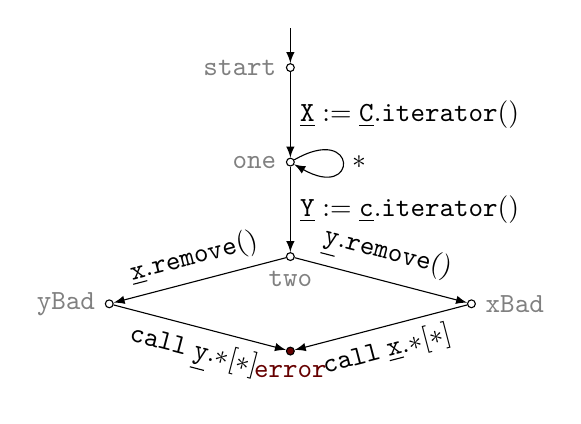
\begin{tikzpicture}
  \def\x{2.3}
  \def\y{1.2}
  \tikzset{vertex/.style={draw,circle,inner sep=1pt}}
  \tikzset{transition/.style={->,>=latex}}
  \tikzset{every label/.style={gray}}
  \node[vertex] (start) at (0,0) [label=left:\texttt{start}] {};
  \node[vertex] (one) at (0,-1*\y) [label=left:\texttt{one}] {};
  \node[vertex] (two) at (0,-2*\y) [label=below:\texttt{two}] {};
  \node[vertex] (xBad) at (1*\x,-2.5*\y) [label=right:\texttt{xBad}] {};
  \node[vertex] (yBad) at (-1*\x,-2.5*\y) [label=left:\texttt{yBad}] {};
  \node[vertex,fill=darkred] (error) at (0,-3*\y) [label=below:\textcolor{darkred}{\texttt{error}}] {};
  \draw[transition] (0,0.5)--(start);
  \draw[transition] (start)--node[right]{$\pattern X:=\pattern C.\mathtt{iterator}()$} (one);
  \draw[transition] (one) .. controls +(30:1cm) and +(-30:1cm) .. node[right]{$*$} (one);
  \draw[transition] (one)--node[right]{$\pattern Y:=\pattern c.\mathtt{iterator}()$} (two);
  \draw[transition] (two) -- node[sloped,above]{$\pattern y.\mathtt{remove}()$} (xBad);
  \draw[transition] (two)--node[sloped,above]{$\pattern x.\mathtt{remove}()$} (yBad);
  \draw[transition] (xBad)--node[sloped,below]{$\mathtt{call}\;\pattern x.{*}[*]$} (error);
  \draw[transition] (yBad)--node[sloped,below]{$\mathtt{call}\;\pattern y.{*}[*]$} (error);
\end{tikzpicture}
\caption{Property {\tt InvalidateOtherIterators} in diagram form.
}
\label{fig:first.topl}
\end{figure}
\paragraph{Heap Shape and Values Sensitive Properties}  % <<<
The following is a TOPL encoding of the property~\eqref{q:concur-it4} in Section~\ref{sec:motivating-examples}.
It reports an error if a list is cyclic or it has the pan-handle shape (i.e.,
there is a lasso at some point). Directives are omitted.
%
{\small
\delimitVerbatim
\begin{Verbatim}[commandchars=\\\{\}]
 property ListNotCyclic
   start -> start: *
   start -> a: \pattern{X} := *.getList()
   a -> a:     \pattern{X} := x.next()
   a -> b:     \pattern{Y} := x.next()
   b -> b:     \pattern{Y} := y.next()
   b -> error: x := y.next()
   a -> error: x := x.next()
\end{Verbatim}
\delimitVerbatim}%
The idea is that this property will bind the property variable $x$ with any possible object in the list, and the $y$ with any possible successors (via the next field) of the current binding of $x$.
Therefore, if there is a lasso, in the list, this will be detected when a new binding of $y$ via a \texttt{b -> b} becomes equal to the binding of $x$.
The transition \texttt{a ->error} detects the case where there is an object pointing to itself. This property shows the importance of re-binding for specification variables. This phenomenon is also shown by  the following property which detects when a dictionary overwrite one of its bindings.
{\small
\delimitVerbatim
\begin{Verbatim}[commandchars=\\\{\}]
 property BadDictionary
   message "dictionary overwrites its bindings"
   observe <Dictionary.*>
   prefix <Dictionary>
   start -> start: *
   start -> written:   \pattern{D}.put(\pattern{K}, \pattern{V})
   written -> written: d.put(k, \pattern{V})
   written -> error:   !v := d.get(k)
\end{Verbatim}
\delimitVerbatim}%
The overwrite is detected by the guard which checks if the value associated with a key $k$ is the same as the original binding recorded in the property variable $v$.

%>>>
\paragraph{Iterating Ropes Data Structures.} % <<<
The property~\eqref{q:concur-it2} from Section~\ref{sec:motivating-examples} can be encoded in TOPL as follows:
%
{\small
\delimitVerbatim
\begin{Verbatim}[commandchars=\\\{\}]
property IterateRopes
  observe <{Itr.next,Concat.make,Str.itr}>
  prefix <{Itr,Concat,Str}>
  start -> start: *
  start -> a:  \pattern{I} := \pattern{S}.itr()
  a -> a: *, \pattern{S} := make(\pattern{s}, *), \pattern{S} := make(*, \pattern{s})
  a -> b: \pattern{J} := \pattern{s}.itr()
  b -> c: \pattern{i}.set(*)
  c -> error: \pattern{j}.next()
  b -> d: \pattern{j}.set(*)
  d -> error: \pattern{i}.next()
\end{Verbatim}
\delimitVerbatim}%
The re-binding in the self-loop {\tt a -> a} combined with {\tt a->a: *} ensure that iterators of sub-collections in the rope are tracked. Therefore,
of two different iterators of two collections sharing some object invalidating `h the error state. 
\\dd{are there other permutation missed by the property?}

%>>>
\paragraph{Property for Taint Info.} % <<<
To check taint information as described by property~\eqref{q:concur-it3} in Section~\ref{sec:motivating-examples} we can use the following
TOPL specification:
{\small
\delimitVerbatim
\begin{Verbatim}[commandchars=\\\{\}]
property TaintCheck
  observe <{Itr.next,Concat.make,Str.itr}>
  prefix <{Itr,Concat,Str}>
  start -> start: *
  start -> a:  \pattern{X} := input()
  a -> a: \pattern{X} := make(\pattern{x}, *), \pattern{X} := make(*, \pattern{x}), (!sani)(*)
  a -> b: sani(\pattern{x})
  a -> error: sink(\pattern{x})
\end{Verbatim}
\delimitVerbatim}%
The specification takes care to track  any tainted substring $x$ used in the rope and report an error if $x$ reaches the sink method.

\paragraph{Singleton Pattern.} 
The last property we present concerns 
the singleton pattern where the instantiation of a class is restricted to one object. It is used when exactly one object is needed to coordinate actions across the system. It can be enforced by the following.
{\small
\delimitVerbatim
\begin{Verbatim}[commandchars=\\\{\}]
property SingletonPattern
  start -> a:  \pattern{I} := getInstance()
  a -> error:  !\pattern{i}:= getInstance()
\end{Verbatim}
\delimitVerbatim}%
The property produce an error is the object obtained by the method {\tt getInstance()} is not the same as the one already bound to the automata variable $i$.

% >>>
% >>>
\section{Implementation} \label{sec:implementation} % <<<
We have implemented the formal framework in a tool\footnote{\url{http://rgrig.github.com/topl}} for checking whether a Java program violates 
TOPL properties.
The tool consists of two parts: a compiler and a checker.
The TOPL compiler ({\tt toplc}) instruments Java bytecode;
The TOPL checker (class {\tt topl.Checker}) monitors the execution and reports violations.
\autoref{architecture} depicts how the compiler and the checker fit together, thus summarizing our runtime checking system.

\begin{figure}[t]
\begin{center}
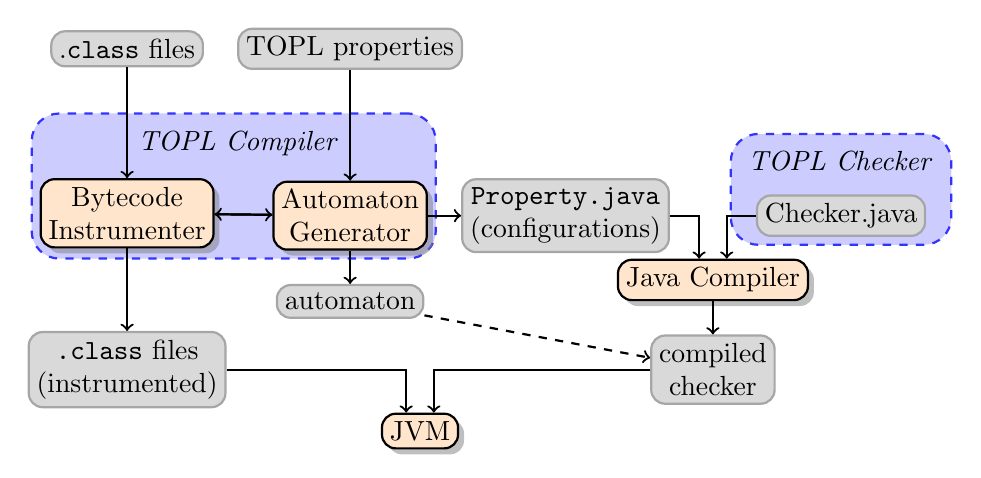
\begin{tikzpicture}[node distance=12pt, auto]
\tikzstyle{system}=[rectangle,
                                draw=blue!80,
                                fill=blue!20,
                                inner sep=0.1cm,
                                rounded corners=10pt,
                                style=dashed,thick]
\tikzstyle{program}=[rectangle,
                                  draw=black,
                                  fill=orange!20,
                                  inner sep=0.1cm,
                                  rounded corners=5pt,
                                  style=thick,
                                  drop shadow]
\tikzstyle{data}=[rectangle,
                            draw=gray!70,
                            fill=gray!30,
                            inner sep=0.1cm,
                            rounded corners=5pt,
                            style=thick]
\node[data] (classes) {{.\tt class} files};
\node[data, right=of classes] (properties) {TOPL properties};

\node[below=of classes] (classesd) {};
\node[below=of properties] (propertiesd) {};

\node[program, below=40pt of classes, align=center] (instrumenter)
  {Bytecode\\Instrumenter};
\node[program, below=40pt of properties, align=center] (genautomaton)
  {Automaton\\Generator};

\node[data, right=of genautomaton, align=center] (javaproperties)
  {{\tt Property.java}\\(configurations)};
\node[data, below=of genautomaton] (automaton) {automaton};
\node[right=of javaproperties] (javadummy) {};
\node[data, right=of javadummy] (checker) {Checker.java};
\node[program, below=of javadummy] (javac) {Java Compiler};

\node[data, below=of javac, align=center] (classproperties)
  {compiled\\checker};
\node[data, align=center] at (instrumenter |- classproperties)
  (instrclasses) {{\tt .class} files\\(instrumented)};
\node at ($(instrclasses)!.5!(classproperties)$) (classdummy) {};
\node[program, below=of classdummy] (jvm) {JVM};

\node[above=5pt] at ($(instrumenter.north)!.5!(genautomaton.north)$) (topllabel) {\emph{TOPL Compiler}};
\node[above=5pt of checker] (checkerlabel) {\emph{TOPL Checker}};
\begin{pgfonlayer}{background}
  \node[system, fit = (topllabel) (instrumenter) (genautomaton)] (TOPLC) {};
  \node[system, fit = (checker) (checkerlabel)] (CHECKER) {};
\end{pgfonlayer}

\path[thick, ->]
(classes) edge (instrumenter)

(genautomaton) edge (instrumenter)
(instrumenter) edge (genautomaton)

(properties) edge (genautomaton)
(genautomaton)  edge (javaproperties)
(javac) edge (classproperties)

(genautomaton) edge (automaton)

(instrumenter) edge (instrclasses);

\draw[thick, ->]
(instrclasses) -| ($(jvm.north)-(5pt,0)$);
\draw[thick, ->]
(classproperties) -| ($(jvm.north)+(5pt,0)$);
\draw[thick, ->]
(javaproperties)  -| ($(javac.north)-(5pt,0)$);
\draw[thick, ->]
(checker)  -| ($(javac.north)+(5pt,0)$);

\draw[thick, ->, dashed]
(automaton) -- (classproperties);
(\end{tikzpicture}

\caption{Architecture of the TOPL tool}
\label{architecture}
\end{center}
\end{figure}

\paragraph{The TOPL Checker.} % <<<
The checker logs the property violations it detects. 
Internally it  maintains a set of active states.
New states are  produced by applying an action to an existing state (called the parent).
For error reporting, each state keeps track of its parent.
The implementation takes advantage of this fact by representing stores
using persistent sets for bindings;  more precisely, we use treaps~\cite{DBLP:conf/focs/AragonS89}.

As states point to their parent, we need some mean to control overhead.  This is done by configurable parameter for 
the history length~$h$ in {\tt Property.java}.
We should then allow the Java~VM to garbage collect states that are not reachable in $h$~steps from some active state.
To do that, after each execution of a transition we could do a BFS traversal with $h$~steps and set to {\tt null} the parent pointer of fringe states.
However, for $n$~active states, the traversal would take $O(nh)$~time.
The procedure for executing transitions takes $O(nd)$~time, where $d$ is the maximum out-degree of the property.
So, the checker would become much slower if $h>d$, which usually is the case.
%
One solution could be to perform the BFS once in every $h/d$~steps.
The solution we implemented tries to better address the average case.
We remember the number~$m$ of states seen by a BFS, and perform the next BFS after $\sim m$~new states were created.

The set of active states in nondeterministic automata can be unbounded.
Therefore, as for the case of trace lengths, we impose a bound on number of active states. 
The bound can be configured by the user  in the {\tt Property.java}  file.  
The  strategy for forgetting states can also be chosen among: {\em random}, {\em newest}, and {\em oldest}.
Newest\slash oldest refer to a time attached to states.
The time  of a state is the number of transitions  taken to reach that state.

% >>>
\paragraph{The TOPL Compiler.} \label{sec:toplc} % <<<
The compiler takes as input a Java project and a set of TOPL properties.
The Java project is defined to be all files in a given directory, recursively descending into jar and zip files as well as  subdirectories.
The compiler produces (1)~a copy of the Java project with the class files instrumented, and (2)~a TOPL automaton.
%The bytecode instrumentation and the construction of the TOPL automaton are intertwined.
Only the Java methods relevant to the given TOPL properties are instrumented, but taking into consideration 
 the inheritance tree of  project.
For example, suppose that a TOPL property mentions the method {\tt next} from the interface {\tt Iterator}.
Then all the methods that implement {\tt Iterator.next} are instrumented and  matched by the automaton.
%
More in details the compiler execute  five phases.
%\begin{enumerate}
First, TOPL properties are converted into a simpler, intermediate format. 
Second, the compiler  {\em staticically checks}  that the property is well-formed (e.g., variables writes must precede reads). We plan to also statically check whether the automaton can never fail.
%
Third,  all properties are merged into one automaton that is  dumped into the file {\tt Property.text}.
%
Fourth, the compiler generates the checker configurations in 
the file {\tt Property.java}. This file contains 
info used by the TOPL property and code configuring the checker.
Configuration parameters include:
\begin{itemize}
\item \emph{History length}---how many events to remember.
  A high value reports more events that led to \error.
  A low value reduces the space and time overhead.
\item \emph{Maximum number of active states}.
  A high value increases the chances of detecting violations at the cost of higher  overhead.

\item \emph{Collect call stacks} is a flag for including/excluding  call stacks in violation reports.
%
\item {\em Approximantion method} gives different ways in which the history informations are forgotten when  the max amount of info 
allowed is reached.
\end{itemize}
%
Fifth, the compiler instruments methods' bytecode.\footnote{To instrument Java bytecode we use a fork of the library 
Barista~\cite{barista}.}

% >>>
% >>>
\section{Experimental Results}\label{sec:results} % <<<

We expect our technique to be most useful during development.
Library writers will document temporal constraints in TOPL, not just in English.

We measure the overhead on the test suite DaCapo~\cite{dblp:conf/oopsla/dacapo}, version~9.12.
DaCapo is a collection of automated tests that exercise large portions of code from open-source projects.
We focus on $3$~projects that are still widely developed and used: Tomcat, H2, and PMD\null.
These are all mature projects with many users.
DaCapo itself was used for many experiments by the research community.
Hence, we do not expect to find any bugs, but aim to measure the overhead.
For each project we write a few TOPL properties that encode informal temporal information that exists in the code comments.

We measure both time and space overhead.
Time overhead is reported  for various configurations of the checker, and  for the original bytecode, with no instrumentation.
%
All experiments are performed on an Intel i5 machine with $4$~cores at $3.33\rm\,GHz$ with  $4\rm\,GiB$ of memory and 
running Linux~2.6.32 and Java VM~1.6.0\_20.


% >>>
\paragraph{A Bug's Death.} % <<<

The interface \texttt{ServletResponse} from Tomcat contains methods \texttt{getWriter} and \texttt{getOutputStream}.
The documentation of \texttt{getWriter} states that ``either this method or \texttt{getOutputStream} may be called to write the body, not both''.
We initially interpreted this comment as follows.
\eqquote{It is illegal to call both the method {\tt getWriter} and the method {\tt getOutputStream} on the same instance of {\tt ServletResponse}.}{eq:prop-ws-strong}
The TOPL checker reported many violations of~\eqref{eq:prop-ws-strong}.
We were not too surprised because we were unsure of the intended meaning of the comment.
We were surprised, however, that sometimes a {\tt null} dereference occurred in DaCapo itself.
We investigated.
The statement that threw a {\tt null}-pointer exception was the following:
\begin{align}\label{eq:npe-src}
\text{\Verb@if (log != null) log.write(b);@}
\end{align}
It must be that a concurrent thread sets {\tt log} to~{\tt null}.
The statement is located in the method {\tt write} of the class {\tt TeeOutputStream}.
The only method that sets {\tt log} to~{\tt null} is {\tt closeLog}, from the same class.
So, we wrote a TOPL property saying that \textit{executions of {\tt write} and {\tt closeLog} must not overlap in time}, and we asked for error reports that include call stacks.
Indeed, DaCapo's main loop sometimes calls {\tt closeLog} while the Tomcat server is printing.

TOPL helped us find a concurrency bug in the infrastructure of DaCapo.
First, the bytecode instrumented by TOPL helped us notice the problem.
The reason is \emph{not} that a certain interleaving became more likely.
Bug~2934521 of DaCapo mentions that exceptions of the Tomcat benchmark are silently ignored.
This is why the {\tt null}-dereference was not noticed before.
The TOPL checker tried to report an unrelated issue to {\tt System.err}.
DaCapo had redirected the standard error stream to its own class, which faulted.
TOPL caught the error and reported it as an internal issue, because no exceptions should be thrown while running the TOPL checker.
Second, TOPL helped us identify the data race.
It would have been more difficult to figure out which threads exactly used the stream simultaneously.

We then tried a weaker version of property~\eqref{eq:prop-ws-strong}:
\eqquote{Stream and writer of a response cannot both be used.}
{eq:prop-ws-weak}
This property\footnote{\url{http://goo.gl/V008y}} involves three related objects.
It turns out this property is also violated.
After reading the code to which the error traces pointed at, we noticed that the comments of some implementing classes weaken the contract:
They say that the stream and the response cannot be used without an intervening {\tt reset}.
In this case the comments on the interface {\tt ServletResponse} are arguably wrong, rather than the code.
This brings out another advantage of TOPL:
Since TOPL properties are processed by tools, they are less likely to become out-of-sync with the code.

% >>>
\subsection{Benchmarks} % <<<
\begin{table*}[t]
\begin{center}
\begin{tabular}{|l|r||r|r||r|r||r|r||r|r|} \hline
  & original  & \multicolumn{2}{|c|}{HasNext} & \multicolumn{2}{c|}{UnsafeIterator} &\multicolumn{2}{|c|}{UnsafeMapIterator} & \multicolumn{2}{|c|}{UnsafeFileWriter}
%  & orig.  & \multicolumn{2}{|c|}{$P_1$} & \multicolumn{2}{c|}{$P_2$} &\multicolumn{2}{|c|}{$P_3$} & \multicolumn{2}{|c|}{$P_4$}
  \\ \hline
  & & st=3 & st=10 & st=3 & st=10 & st=3 & st=10 & st=3 & st=10 
  \\ \hline \hline
 avrora  & 8.1 & 27.8 & 60.5 & 163.3 & 323.1 & 194.5  & 179.9 & 8.3 & 5.9 
 \\ \hline
 batik     &  1.2  & 18.1 &    3.0 & 3.8 &  3.8  & 3.1 &  3.3 & 1.3  &  1.2 
 \\ \hline
eclipse   &  15.6  &  22.4 &  12.2X & 27.0 &  149.9X & 27.56 &  12.8X & 21.6 &  23.4 
\\ \hline
fop    &   0.3   &  0.9 &  1.9 & 3.5  &  3.6   & 2.7 &   2.7 & 0.3 &   0.3
\\ \hline
h2     &    6.2  &  5.9 &  6.8   & 8.3    & 20.0  & 13.5 & 11.2   & 6.4 & 6.0  
\\ \hline
jython    &  1.9  & 19.8 &  46.1 &  81.5   & 83.0  &  62.8 &       62.7    & 1.9 & 1.8 
\\ \hline
luindex     &  0.8   & 0.8 &   0.8    & 0.8 & 0.9  & 1.0  &   0.9 & 0.8 & 0.9 
\\ \hline
lusearch    &  1.5  &  1.5 &   1.5 & 15.0 &  16.0    & 13.8  &  12.8    & 1.5 & 1.7 
\\ \hline
pmd        &   3.1    & 19.9 & 42.6  &  93.5 & 240.3   & 102.6 &       105.6  & 3.2 &           3.3 
\\ \hline
sunflow    &  3.9   & 3.8 &  3.9  &  4.0 & 3.8    & 3.9 &        3.9     & 3.9 &         4.3 
\\ \hline
tomcat     &   2.5    & 4.2 & 8.3   & 22.9 & 50.9   & 30.0 &        31.0   & 2.6 &          2.7 
\\ \hline
%tradebeans  &  5475  &  XX &     XX  & XX &    XX     & XX &          XX    & XX &           XX 
%\\ \hline
%tradesoap   & 6937   &  XX &    XX    & XX &  XX       & XX &       XX       & XX &        XX   
%\\ \hline
xalan      &    1.5   &  14.5      & 7.1 & 425.0  & 360.9 &  272.0   & 276.5 &  1.5 & 1.2 
\\ \hline  
\end{tabular}
\end{center}
\caption{Experiment on small properties run on the DaCapo benchmarks
  (run in convergence mode). Times are in seconds.}
\label{tab:javamop-experiments}
\end{table*}%

\rg{TODO: Add the JDK properties from JavaMOP people.}
\rg{TODO: Clearly explain that our active configurations (not states, BTW) are \emph{not} the same at all with the number of monitors reported by the other runtime verification people.}

All three benchmarks are large open-source projects with many users and active developers.
The versions were current in 2009 when DaCapo-9.12 was released.

\paragraph{Tomcat 6.0.20.}
Tomcat is a highly concurrent servlet server. 
Servlets are Java programs running in a webserver, extracting data from {\tt ServletRequest}s , and sending data to {\tt ServletResponse}s.
A response has two associated incoming channels: a stream and a writer. Both should not be used concurrently.
%Property~\eqref{eq:prop-ws-strong} is a strong interpretation of this constraint;
%property~\eqref{eq:prop-ws-weak} is a weak interpretation of this constraint.
A response could be forwarded once the servlet sent data to it.
But the servlet, before forwarding the response, must call {\tt flush} on the stream, on ther writer, or on the response itself.
This is the other property we checked.

\paragraph{H2 1.2.121.}
H2 is a database server.
We checked four properties for it.
Three properties express constraints on the order in which the methods of an interface may be called.
For example, a client should not attempt to ask for a row from a cursor that did not advance;
that is, for the interface {\tt Cursor}, the method {\tt next} must be called before calling method {\tt getSearchRow}.
The fourth property describes the contract of the class {\tt SysConstants}.
This class reads environment variables when it is loaded.
Its comments say that it is legal for a program to set these environment variables using the method {\tt System.setProperty}, provided that this is done before the Java VM loads the class {\tt SysConstants}.
It is easy to specify this property because TOPL intentionally treats the special methods {\tt <init>} and {\tt <clinit>} as if they are normal methods.

\paragraph{PMD 4.2.5.}
PMD looks for bugs, dead code, and a few other problems in Java code.
We checked five properties for it.
One of the five involves two objects:
A scope should be asked what is the definition of a name only if it already replied that it knows the name.

% >>>
\subsection{Overhead} % <<<

Instrumenting DaCapo, which has $160\rm\,MiB$, f or a given set of properties takes $7$~minutes.
A change of a runtime parameter, such as the maximum number of tracked active states
does not require re-instrumenting (only recompilation of the TOPL checker).

\paragraph{Space.}
Estimates of heap size showed no significant increase in memory use.
We used a simple method.
The heap of a Java program has three parts: used, garbage, and free.
The class {\tt Runtime} from the package {\tt java.lang} provides an estimate of the total size and of the free size.
The difference is an estimate of the used size, provided the garbage was collected immediately before.
We put this code, which estimates memory use, in the TOPL checker.
So, strictly speaking we did not estimate the memory use without the checker.
However, we used as a baseline a run that tracked no active state.
We also run the estimate for various other counts of tracked active states.

\paragraph{Time.}
\autoref{table:overhead} summarizes the experimental results.
The reference column shows the running time without any instrumentation.
A timeout signifies a time greater than the reference time~$\times100$.
All reported times are averaged over $10$~runs, and are accompanied by the unbiased estimate of standard deviation.
In theory the set of active states is unbounded, but we impose a size limit on it.
The table reports the running times for the instrumented bytecode when the size limit is $0$, $10^1$, $10^2$.
%
%For tomcat the running time is essentially the same when tracking $\le10^4$ active states as it is when tracking $\le10^3$ active states.
%This indicates that $\le10^3$ active states already exhaustively check the given properties.
For h2 the running time is more than $\times1.4$ the reference time even when the TOPL checker is not tracking any active state.
This indicates that we instrumented a simple method that runs often.

\begin{table}[t]\centering
\begin{tabular}{@{}rr@{}lr@{}lr@{}lr@{}lr@{}lr@{}l}
  &&
  & \multicolumn{10}{c}{Number of tracked active states} \\ \cmidrule{4-13}
& \multicolumn{2}{c}{reference}
  &\multicolumn{2}{c}{$\le0$}
  &\multicolumn{2}{c}{$\le10^1$}
  &\multicolumn{2}{c}{$\le10^2$}
%  &\multicolumn{2}{c}{$\le10^3$}
%  &\multicolumn{2}{c}{$\le10^4$} 
\\ \midrule
tomcat
  & $5.3$ & $\pm0.1$
  & $5.4$ & $\pm0.1$
  & $5.6$ & $\pm0.2$
  & $9.0$ & $\pm0.3$
%  & $43.5$ & $\pm1.2$
%  & $43.9$ & $\pm1.0$ 
\\
pmd
  & $5.2$ & $\pm0.4$
  & $5.4$ & $\pm0.2$
  & $12.2$ & $\pm0.3$
  & $47.7$ & $\pm10.7$
%  & \multicolumn{2}{c}{timeout}
%  & \multicolumn{2}{c}{timeout}
  \\
h2
  & $6.6$ & $\pm0.2$
  & $9.5$ & $\pm0.2$
  & $130.1$ & $\pm12.2$
  & \multicolumn{2}{c}{timeout}
%  & \multicolumn{2}{c}{timeout}
%  & \multicolumn{2}{c}{timeout}
  \\
\end{tabular}
\caption{
  Experimental Results.
  Times are in seconds, averaged over $10$~runs.
}\label{table:overhead}
\end{table}

% >>>
% >>>
\section{Related Work}\label{sec:related} %<<<

TOPL is an application of automata theory to program verification.
Consequently, there is related work in the area of automata theory and  in  program verification.

TOPL automata are a variant of {\it register automata\/}~\cite{dblp:conf/focs/kaminskif90}, which were introduced in~1990.
We proved that several decidability results known for register automata also hold for TOPL automata.
Register automata work with infinite alphabets, as do a few other types of automata~\cite{dblp:conf/csl/segoufin06}.
Until now, such automata found applications mostly related to databases and XML\null.
Intuitively, however, such models are a good fit for expressing properties of programs because the set of program values is infinite.
For example objects could be instantiated inside non-terminating loops.
Our paper exhibits a working runtime verification system based on register automata, thus validating the intuition.

Related work from the area of program verification splits by time of checking (runtime or static) and by programming paradigm (object-oriented or functional).
The work on runtime verification of object-oriented programs is closest to TOPL\null.

{\it JavaMOP\/}~\cite{dblp:journals/sttt/meredithjgcr12} and {\it tracematches\/}~\cite{dblp:conf/oopsla/allanachklmsst05} are the main runtime verification systems that handle multiple objects.
They differ in many details, but the essential ideas fit a common intuition.
To communicate this intuition we depart from the terminologies of \cite{dblp:journals/sttt/meredithjgcr12}~and~\cite{dblp:conf/oopsla/allanachklmsst05}.
The alphabet is~$\Sigma=C\times V$, where $C$~is a finite set of constants and $V$~is an infinite set of values.
The task is to build a recognizer $\Sigma^*\to\B$.
Both approaches build upon a basic recognizer $C^*\to\B$ over finite alphabets.
Tracematches specify this recognizer by regular expressions, while JavaMOP supports several other logics.
Both approaches make further assumptions on the structure of~$V$, and then define a way to specify a family $P\subset\Sigma\to\B$ of predicates over letters.
Each such predicate~$p\in P$ determines a slice $\tau_p\in C^*$ of the trace $\tau\in\Sigma^*$ by retaining exactly those constants from letters satisfying~$p$.
The trace~$\tau$ is recognized when any of its slices satisfy the basic recognizer.
Within such a framework, it seems difficult to express some of our examples, which naturally use an unbounded number of assignments to registers.

Any algorithm that analyzes or transforms JavaMOP properties must be specific to a certain plugin because the formalization of the framework~\cite{dblp:journals/corr/abs-1112-5761} imposes no constraint on recognizers $C^*\to\B$.
In contrast, any algorithmic result discovered for register automata implies one for TOPL properties.
For example we know that the emptiness problem is decidable, and we know that it is impossible to compute the negation of a property.

{\it Tracematches\/}~\cite{dblp:conf/oopsla/allanachklmsst05} are likely to have the same expressivity as JavaMOP with the plugin for regular expressions.
But, we are unaware of a fully formal comparison.
Tracematches evolved from the work on aspect-oriented programming.
Unsurprisingly, the user may specify arbitrary code to run when a match is found.
The formal semantics ignore this arbitrary code and how it could influence further matches.

{\it QVM\/}~\cite{arnold:2008} is a runtime monitoring system tracking a subset of objects, chosen by
sampling. To ensure that the timing overhead of the monitoring is below a given target, the sampling rate is 
automatically adapted on the fly. For TOPL the control of the overhead is done manually by  the programmer who can tune the quantity of info to be tracked.
To improve performance,  the implementation of the QVM monitor is in the virtual machine, which, as a consequence makes it less portable for
different virtual machines. 

{\it ConSpec\/}~\cite{DBLP:journals/entcs/AktugN08} is a language used to describe security policies.
Because ConSpec automatons are deterministic and have only a countable number of states, they cannot in principle express the property \texttt{InvalidateOtherIterators} (\autoref{sec:examples.steps}).

From the techniques used mostly for static verification of object-oriented programs, {\it typestates\/}~\cite{strom1986} are probably most similar to TOPL\null.
A modular static verification method for typestate protocols is introduced in~\cite{dblp:conf/oopsla/bierhoffa07}.
The specification method is based on linear logic and relations among objects in the protocol are monitored by a tailored system of permissions.
The specification of the interactions among objects by means of permissions adds an extra level of machinery which increases the gap between the intuitive protocol description and its formalization.
Similarly~\cite{deline2004,dblp:conf/sigsoft/BierhoffA05} provide a mean to specify typestate properties that belong to a single object.
The specified properties are reminiscent of contracts or pre/post-conditions for methods and can deal with inheritance.
In~\cite{dblp:conf/issta/FinkYDRG06} the authors present sound verification techniques for typestate properties of Java  programs.
Their approach is divided in several stages with different verifiers varying for cost and precision.
In the early stages efficient but imprecise analyses are employed whereas more expensive and precise techniques are then progressively employed in later stages.
Every stage focuses on verifying only the parts of the code that previous stages failed to verify.
It is likely that  TOPL could be fruitfully combined with their analysis technique.

A specification language for interface checking aimed at C programs (called SLIC) is introduced in~\cite{ball2002}.
Differences between SLIC and TOPL include: the use (in SLIC) of non-determinism to encode universal quantification of dynamically allocated data, and the  ability to have complex code in the automaton transitions.
TOPL specifications naturally express universally quantified properties over data structures and for computability reasons,  we have chosen to limit the  actions performed during automaton transitions.
Simple SLIC specifications are verified by  the SLAM verifier~\cite{dblp:conf/cav/ballr01}.
While SLAM specialises on device drivers and checks client conformance rather than full protocols,
very general specifications of object-oriented program behaviour can be given in JML~\cite{jml} and Spec$\sharp$~\cite{DBLP:journals/jot/BarnettDFLS04}. However the latter two languages focus on class specifications and do not have temporal features.

Finally, there are similar investigations going on in the functional programming community.
In~\cite{disney2011} contracts are used to express legal traces of programs in a functional language with references.
The contracts specify traces as regular expressions over calls and returns, and hence, they resemble our automata, in a quite different setting.
Here, the specifications are function-centered, though, and again, capturing inter-object relations seems somewhat tricky.

% >>>
\section{Conclusions and Future Work}\label{sec:conclusions} %<<<
In this paper we have introduced TOPL a new runtime verification system aimed at checking temporal safety properties of object-oriented programs. 
For TOPL we have defined solid formal foundations based on register automata. Moreover we have studied the formal correspondence between TOPL automata and register automata proving that they are equally expressive.
TOPL has been implemented in a practical tool that we have applied  to a variety of programs including large open source Java projects.
%

%\paragraph{Future work.}
In the future, we intend to combine TOPL with  separation logic~\cite{reynolds2002} in order to deal with the heavy use of the heap and aliasing in object-oriented software.
Moreover, we aim at developing static analysis techniques for TOPL properties using the jStar framework~\cite{DBLP:conf/oopsla/DistefanoP08}.
This will require investigating suitable abstraction for obtaining meaningful and precise over-approximations of the state space of the programs.
Finally, we intend to develop a tailored bi-abduction inference technology~\cite{dblp:conf/popl/CalcagnoDOY09} which would help with scalability of the analysis.

%>>>
\bibliographystyle{abbrv} % and appendix <<<
\bibliography{safety}

% \appendix
% \section{TOPL Syntax}
% \label{app:syntax}
% \begin{tabular}{l}
% \grammar{
%   Property& \b{property} Identifier Item\* \cr
%   Item& Prefix \| Observe \| Transition \cr
%   Prefix& \b{prefix} \b< StringPattern \b> \cr
%   Observe& \b{observe} \b< StringPattern \b> \cr
%   Transition& Arc \b: Label \(\b, Label\)\* \cr
%   StringPattern& \(Letter \| \b. \| \b* \| \b{\{} \| \b{\}} \| \b, \)\+ \cr
%   Arc& Vertex \b{->} Vertex \cr
%   Label& Tag\? MethodPattern \cr
%   Vertex& Identifier \cr
%   Tag& \b{call} \| \b{return} \cr
%   MethodPattern& ResultPattern\? NamePattern ArgumentsPattern \cr
%   ResultPattern& ValuePattern \b{:=} \cr
%   NamePattern& StringPattern \cr
%   ArgumentsPattern& \b( \(ValuePattern \(\b, ValuePattern\)\*\)\? \b) \cr
%   ArgumentsPattern& \b[ IntegerPattern \b] \cr
%   ValuePattern& \b* \| \b< Literal \b> \| UppercaseId \| LowercaseId \cr
%   IntegerPattern& \b* \| IntegerLiteral \cr
% }
% \end{tabular}

%
%\begin{figure*}[h]\label{fig:tomcat-prop}
%\begin{Verbatim}
%property InterleavedResponse2
%  // vertex names: w = got writer; W = used writer; similarly for s, S
%  message "Incompatible methods for putting data into a response were used."
%  observe <javax.servlet.ServletOutputStream.*>
%  observe <java.io.PrintWriter.*>
%  observe <javax.servlet.ServletResponse.{getOutputStream,getWriter}>
%  prefix <javax.servlet.ServletResponse>
%  start -> start: *
%  start -> w: W := R.getWriter()
%  start -> s: S := R.getOutputStream()
%  w -> sw: S := r.getOutputStream()
%  s -> sw: W := r.getWriter()
%  w -> W: w.*
%  sw -> sW: w.*
%  s -> S: s.*
%  sw -> Sw: s.*
%  W -> sW: S := r.getOutputStream()
%  S -> Sw: W := r.getWriter()
%  sW -> error: s.*
%  Sw -> error: w.*
%\end{Verbatim}
%\caption{Example Tomcat Propery}
%\end{figure*}

% >>>
\end{document}
%% vim:spell errorformat=%f\:%l-%m,%f\:%l\:%m,%f\:%m
%% vim:fmr=<<<,>>>:
